\documentclass[12pt,a4paper]{article}
\usepackage[utf8]{inputenc}
\usepackage[T1]{fontenc}
\usepackage[ngerman]{babel}
\usepackage{graphicx}
\usepackage{hyperref}
\usepackage{geometry}
\usepackage{titlesec}
\usepackage{color}
\usepackage{fancyhdr}
\usepackage{enumitem}
\usepackage{subcaption}
\usepackage{float}
\usepackage{tabularx}
\usepackage{booktabs}
\geometry{left=3cm,right=2.5cm,top=2.5cm,bottom=2.5cm}
\pagestyle{fancy}
\fancyhf{}
\fancyfoot[C]{\thepage}

\title{\textbf{Dokumentation – Software Engineering\\App Palabra}}
\author{Marit Z., Erik D., Daniel H.}
\date{}

\begin{document}

\maketitle

\tableofcontents
\newpage

\section{Einleitung}

\subsection{Projektumfeld}
Im Rahmen des Software-Engineering-Unterrichts wurde die Entwicklung und Umsetzung einer App durchgeführt. Diese Dokumentation beschreibt die Vorgehensweise bei der Entwicklung der App „Palabra“. Zunächst werden das Projektziel und die Anforderungen erläutert. Anschließend folgen die Analyse der Idee sowie die Definition der Soll- und Wunschkriterien. Im Entwurfsabschnitt werden die Auswahl der Zielplattform und des Architekturmodells begründet, das Design der Benutzeroberfläche vorgestellt und die getroffenen Designentscheidungen erläutert. Dies wird durch Screenshots, Mockups und Farbpaletten ergänzt. Weiterhin werden die Datenstrukturen anhand des ER-Modells, Klassen-, Objekt-, Sequenz- und Struktogrammen sowie des Programmablaufplans dargestellt, um die Funktionen der App anschaulich zu machen. Im Implementierungsabschnitt wird das Vorgehen bei der Entwicklung beschrieben, insbesondere die Erstellung der Benutzeroberfläche und die Implementierung der Datenbank, unterstützt durch Klassendiagramme. Abschließend erfolgt eine Reflexion des Projekts, ein Soll-Ist-Vergleich sowie ein Ausblick auf mögliche Erweiterungen.

\subsection{Projektziel und Kurzbeschreibung}
Ziel des Projekts ist die Entwicklung einer Lern-App zum Vokabellernen. Beim Start der App kann der Nutzer zwischen den Optionen „Lektionen auswählen“, „zufällige Vokabelabfrage“ und „Abfrage aller Vokabeln“ wählen. Die Lektionen-Übersicht zeigt alle vom Nutzer erstellten Lektionen; dort können Lektionen erstellt, gelöscht oder gestartet werden. Beim Start einer Lektion erscheint jeweils eine Vokabel mit drei Antwortmöglichkeiten, von denen eine korrekt ist. Nach Auswahl der richtigen Antwort wird dies angezeigt und die nächste Vokabel erscheint. Während der Abfrage kann der Nutzer jederzeit die aktuelle Vokabelliste einsehen. Die Option „zufällige Abfrage“ fragt zufällig ausgewählte Vokabeln aus allen Listen ab; die Option „alle Vokabeln abfragen“ prüft sämtliche gespeicherten Vokabeln.

\subsection{Organisation}
Die Aufgabenverteilung erfolgte nach den jeweiligen Stärken und Interessen der Teammitglieder. Erik war als Head Programmer ausschließlich für den Code verantwortlich. Marit übernahm Dokumentation und Design. Daniel arbeitete als Allrounder sowohl am Code als auch an der Dokumentation mit.

Wichtige Abgabetermine wurden in Notion dokumentiert und organisiert. Für jede Aufgabe wurde eine eigene Seite erstellt und einer verantwortlichen Person zugewiesen. Tagesprotokolle wurden ebenfalls in Notion hochgeladen, sodass der Fortschritt für alle Teammitglieder transparent war. Dadurch verlief die Organisation reibungslos, und größere Komplikationen konnten vermieden werden.

\section{Planung}

\subsection{Projektphasen und Zeitplanung}
Die Zeitplanung orientierte sich an festgelegten Meilensteinen. Wichtige Termine, wie die Abgabe der Fachkonzeptklassen, wurden als Meilensteine definiert. Aufgaben wurden in die Kategorien „Nicht begonnen“, „In Bearbeitung“ und „Erledigt“ unterteilt, um den Fortschritt übersichtlich zu gestalten.

Zudem wurden alle auftretenden Probleme in einer Tabelle dokumentiert, um deren Nachvollziehbarkeit zu gewährleisten und den Zeitpunkt sowie die Lösung festzuhalten.

\subsection{Ressourcenplanung}
Das Projektteam bestand aus drei Mitgliedern mit klar abgegrenzten Verantwortlichkeiten.

\begin{itemize}
    \item \textbf{Erik D. (Head Programmer):} Technische Umsetzung der App, Implementierung der Kernfunktionen, Integration neuer Features und Durchführung von Tests. Entwicklung mit Android Studio und Kotlin. Versionsverwaltung über GitHub.
    \item \textbf{Daniel H. (Allrounder):} Koordination und Organisation, Planung und Überwachung der Arbeitsschritte, Unterstützung beim Testen und bei der Dokumentation. Projektmanagement und Kommunikation über Notion.
    \item \textbf{Marit Z. (UI-Design):} Entwurf benutzerfreundlicher Layouts, Entwicklung von Mockups und Umsetzung des Designs in Android Studio. Fokus auf intuitive Bedienung und konsistentes Erscheinungsbild.
\end{itemize}

Die Dokumentation wurde gemeinsam mit LaTeX erstellt. Zentrale technische Ressourcen waren GitHub (Versionskontrolle), Android Studio (Entwicklungsumgebung), Kotlin (Programmiersprache), Notion (Projektmanagement) und LaTeX (Dokumentation).

\subsection{Entwicklungsprozess}
Die Entwicklung der App \textit{Palabra} erfolgte iterativ und teamorientiert unter Einsatz moderner Softwareentwicklungsmethoden. Android Studio mit Kotlin wurde als Entwicklungsumgebung genutzt, die Versionskontrolle erfolgte über GitHub.

Die Aufgabenverteilung war klar strukturiert:
\begin{itemize}
    \item \textbf{Erik D.:} Planung, Implementierung und Pflege der Kernfunktionen. Erstellung und Bearbeitung von Issues auf GitHub.
    \item \textbf{Daniel H.:} Überwachung der Commits und Issues, Implementierung von Lösungen bei technischen Problemen, Dokumentation wichtiger Änderungen.
    \item \textbf{Marit Z.:} Design und Überarbeitung des App-Layouts, Optimierung des Stylings und Anpassungen wie der Dark Mode.
\end{itemize}

Der Entwicklungsprozess umfasste regelmäßige Code-Reviews, Nutzung von GitHub-Issues zur Aufgabenverwaltung und enge Teamabstimmung. Features wurden schrittweise umgesetzt, getestet und verbessert. Wichtige Meilensteine und Änderungen wurden durch aussagekräftige Commits dokumentiert.

\subsubsection{Wichtige Commits}
Im Folgenden sind die wichtigsten Commits mit Link zum Repository aufgeführt. Diese Liste dokumentiert die Entwicklungsschritte und zeigt, wie sich das Projekt technisch und funktional weiterentwickelt hat:

\begin{itemize}
    \item \href{https://github.com/Erik-Donath/Palabra/commit/864ebf0f71aac98fae10cba9fc118028a1333fd8}{Initial commit} -- Projektstart und erste Strukturierung des Repositories.
    \item \href{https://github.com/Erik-Donath/Palabra/commit/13b34d5efca6c7f2dcc97147ada92919e193a322}{Added Room Library und Projektarchitektur} -- Integration der Room-Datenbank und grundlegende Architektur.
    \item \href{https://github.com/Erik-Donath/Palabra/commit/0d82f5896756da601495fac90b8f8a05eca06a81}{Replaced Intent Solution with ViewModels} -- Umstellung auf MVVM-Architektur mit ViewModels.
    \item \href{https://github.com/Erik-Donath/Palabra/commit/11be0359de673b3c92dd18909bb47f754bcf3040}{Add License Activity} -- Hinzufügen einer Lizenzanzeige.
    \item \href{https://github.com/Erik-Donath/Palabra/commit/507cadc495cdee66976928d968aa23b10c6f086d}{Updated Kotlin; Simplified Code; Added Back Button support} -- Aktualisierung der Kotlin-Version und Verbesserung der Navigation.
    \item \href{https://github.com/Erik-Donath/Palabra/commit/c65171940fad9fe11f5604990ea31395d8c1b829}{Rewritten Database} -- Komplette Überarbeitung der Datenbankstruktur.
    \item \href{https://github.com/Erik-Donath/Palabra/commit/56ce6556d47316994946e8291166b68bd2bec3f9}{Added Flags} -- Implementierung von Flaggen zur Sprachunterstützung.
    \item \href{https://github.com/Erik-Donath/Palabra/commit/bc822c0f34fbeec6566a5ba35a1defa666dad456}{Fixed Country and Lang Codes; Remove unused imports} -- Fehlerbehebungen bei Ländercodes und Codebereinigung.
    \item \href{https://github.com/Erik-Donath/Palabra/commit/a31289a9ef71628d3ffa6170a53dae528de9d0e5}{Added new Vocab and new Lektion Dialogs} -- Neue Dialoge zum Hinzufügen von Vokabeln und Lektionen.
    \item \href{https://github.com/Erik-Donath/Palabra/commit/a846ee02333d85817c9655c5fd34cc9a7acabd9d}{Rewritten Learn Activity and Implemented Debug Provider} -- Überarbeitung der Lern-Activity und Debugging-Tools.
    \item \href{https://github.com/Erik-Donath/Palabra/commit/bd11641738224ec701efae7cd1243153af7b10fe}{Removed unused Flags and reordered Languages after global popularity} -- Optimierung der Sprachunterstützung.
    \item \href{https://github.com/Erik-Donath/Palabra/commit/6e4982769e27744cca8d112e1807f76f4ff160de}{Added German translation} -- Ergänzung einer deutschen Übersetzung.
    \item \href{https://github.com/Erik-Donath/Palabra/commit/4bc28a645fe7c87899ccc57ef4d8a160bfef4d85}{Added Dark Mode support} -- Einführung des Dark Modes.
    \item \href{https://github.com/Erik-Donath/Palabra/commit/bf8beefcf7cca51e4da28855030c7488e79f9806}{Removed Languages that are not writable with the standard keyboard} -- Anpassung der Sprachoptionen.
    \item \href{https://github.com/Erik-Donath/Palabra/commit/3b6bec27e538deed545c870dd79b3046855a1120}{Added Hack to check if no vocabs available before initializing AllProvider} -- Fehlerbehandlung bei leerer Datenbank.
    \item \href{https://github.com/Erik-Donath/Palabra/commit/2a7ab3cd174015657479552cb8bf8bb52b9a2f8b}{Added AllProvider} -- Einführung des AllProviders zur Vokabelverwaltung.
    \item \href{https://github.com/Erik-Donath/Palabra/commit/525dcb48f3128b1463a836a1db68a558072ab39c}{Added LektionProvider} -- Einführung des LektionProviders.
    \item \href{https://github.com/Erik-Donath/Palabra/commit/51ced0c599b4e4707231b10cbceea484b169148a}{changed color (UI-Verbesserung)} -- Verbesserungen am Farbschema.
    \item \href{https://github.com/Erik-Donath/Palabra/commit/5cb0c4cd391b8ec789e4889fd4ed4bf5be747797}{Rename Ressource files} -- Umbenennung von Ressourcen für bessere Übersicht.
    \item \href{https://github.com/Erik-Donath/Palabra/commit/b1787998fa5c91b92e6411b9339e7b51cbdd347b}{Added LektionActivity} -- Neue Activity für Lektionen.
    \item \href{https://github.com/Erik-Donath/Palabra/commit/39da77321c858532260274ccc76ad0458cea806d}{Added Vocab List to each Lektion} -- Vokabellisten für jede Lektion.
    \item \href{https://github.com/Erik-Donath/Palabra/commit/7f204528d8f7df18da4316c6c8b84396d3c45299}{Added Delete Buttons} -- Löschfunktionen für Vokabeln und Lektionen.
\end{itemize}

\subsubsection{Release 0.5 (Alpha)}
Die zum Zeitpunkt der Dokumentation aktuelle Version ist unter \href{https://github.com/Erik-Donath/Palabra/releases/tag/0.5}{Github Release 0.5} verfügbar.

\subsection{Testdokumentation}
Die App wurde durch manuelle Tests auf verschiedenen Android-Geräten geprüft. Es wurden insbesondere folgende Funktionen getestet:
\begin{itemize}
\item Erstellen, Löschen und Starten von Lektionen
\item Abfrage und Bewertung von Vokabeln
\item Navigation zwischen den Ansichten
\item Speicherung und Wiederherstellung von Daten nach App-Neustart
\end{itemize}
Automatisierte Unit-Tests sind für die Datenbankfunktionen in Planung.

\section{Analyse}

\subsection{Soll-Analyse}
Im Rahmen der Soll-Analyse wurden die zentralen Funktionen definiert, die in der ersten Umsetzungsphase realisiert werden sollten. Im Vordergrund standen Benutzerfreundlichkeit und eine effektive Unterstützung beim Vokabellernen.

Nach dem Start der App kann der Nutzer auf einer übersichtlichen Startseite zwischen verschiedenen Abfrageoptionen wählen: lektionsbasierte Abfrage, intelligente Abfrage (schlecht gelernte Vokabeln werden priorisiert) und die Abfrage aller gespeicherten Vokabeln.

Ein Score zeigt dem Nutzer, wie viele Vokabeln er richtig beantwortet hat, um die Motivation zu steigern und den Lernfortschritt zu visualisieren.

Der Nutzer kann seine gespeicherten Vokabeln einsehen. Bei den Lektionen ist es möglich, neue Lektionen zu erstellen und bestehende zu löschen, um die App individuell anzupassen.

Ein Button ermöglicht die Einsicht in die verwendete Open-Source-Lizenz der App.

\subsubsection{Anwendungsfalldiagramm}
\begin{figure}[H]
    \centering
    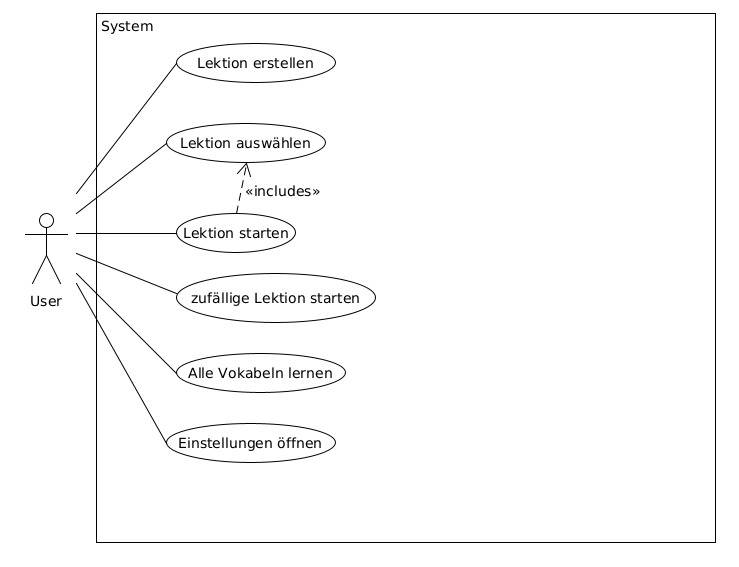
\includegraphics[width=0.7\textwidth]{use-case-diagramm.jpeg}
    \caption{Anwendungsfalldiagramm}
    \label{fig:festes_bild}
\end{figure}

\subsection{Wunschkriterien}
Wunschkriterien umfassen die Möglichkeit, Vokabellisten zu importieren und zu exportieren, um eigene Sammlungen zu teilen oder bestehende Listen zu nutzen. Eine Funktion zur Konjugation von Verben soll verschiedene Verbformen abbilden und abfragen. Die Bereitstellung der App für iOS wird angestrebt, was einen Umstieg auf ein plattformübergreifendes Framework wie Flutter erfordern würde. Ein Dark Mode wird ebenfalls als wünschenswert betrachtet.

\section{Entwurf}

\subsection{Zielplattform}
Als Zielplattform wurde Android (mobil) gewählt, da Smartphones allgegenwärtig sind und Android das weltweit meistgenutzte mobile Betriebssystem ist. Die Entwicklung erfolgte mit Kotlin in Android Studio, was durch offizielle Unterstützung und moderne Sprachfeatures die Teamarbeit erleichtert.

Für die Datenbank kam die Room Persistence Library als Wrapper für SQLite zum Einsatz. Diese ermöglicht eine performante und speichereffiziente Verwaltung der Lektionen und Vokabeln.

\subsection{Architekturdesign}
Das Architekturdesign folgt dem MVVM-Pattern (Model-View-ViewModel). Die Datenmodelle werden durch Room-Entities wie \texttt{Lektion} und \texttt{Vocab} realisiert. Zugriff und Persistenz erfolgen über DAOs (Data Access Object) und ein zentrales Repository, welches die Datenhaltung von Logik und Darstellung trennt.

Die ViewModels, z.B. das \texttt{LektionViewModel}, sind das Bindeglied zwischen UI und Datenhaltung. Sie verwalten den Zustand der UI und liefern die benötigten Daten als LiveData an die View-Komponenten. Die ViewModels werden über Factories erzeugt, was die Testbarkeit verbessert.

Die Benutzeroberfläche besteht aus Activities und Adaptern (z.B. \texttt{MainActivity}, \texttt{LektionActivity}, \texttt{LektionAdapter}), die für die Darstellung und das UI-Handling zuständig sind. Sie beobachten die ViewModels und reagieren mittels Observer-Pattern auf Datenänderungen. Die UI wird mit XML-Layouts, ViewBinding und DataBinding gestaltet.

\subsection{Benutzeroberfläche}
Die Benutzeroberfläche ist schlicht und minimalistisch gehalten, sodass die App klar und einfach zu verstehen ist. Dafür wurde ein helles, freundliches Farbschema gewählt, bei dem besonders auf gute Lesbarkeit der Schrift – zum Beispiel in Buttons – geachtet wurde. Die beiden Hauptfarben sind Schwarz und Weiß. Als Kontrastfarben kommen ein dunkles Blau und ein Beige zum Einsatz. Ergänzt wird das Farbschema durch die Signalfarben Rot und Grün, die sich durch das gesamte Design der App ziehen. Der Hintergrund ist weiß, die Schrift schwarz. Buttons, die zum Löschen oder Starten verwendet werden, nutzen die Signalfarben.

\begin{figure}[h]
    \centering
    \begin{subcaptionbox}{Farbschema\label{fig:bild1}}[0.45\linewidth]
        {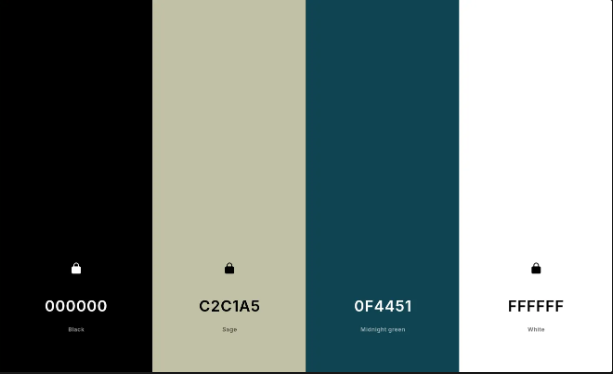
\includegraphics[width=\linewidth]{Farbschema.png}}
    \end{subcaptionbox}
    \hfill
    \begin{subcaptionbox}{Signalfarben\label{fig:bild2}}[0.30\linewidth]
        {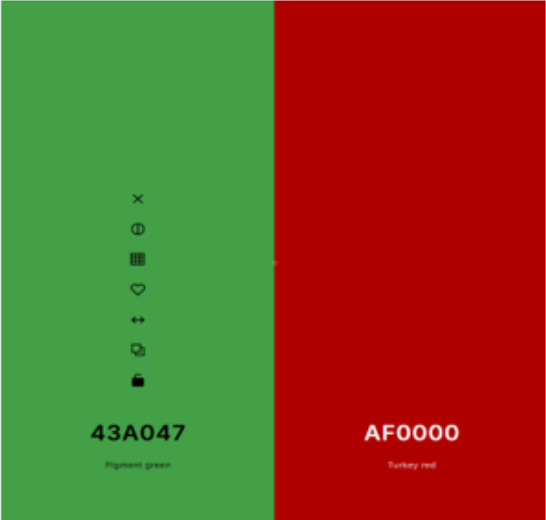
\includegraphics[width=\linewidth]{Signalfarben.png}}
    \end{subcaptionbox}
    \caption{Farbschemen der App}
    \label{fig:nebeneinander}
\end{figure}

Die Menüführung erfolgt über Buttons. Alle wichtigen Elemente erhalten einen Button, der durch die Akzentfarbe Dunkelblau auf dem weißen Hintergrund gut sichtbar ist. Das Grundkonzept sieht vor, dass die Hauptauswahlen als drei Buttons untereinander angeordnet sind – sowohl auf der Startseite als auch bei der Vokabelabfrage.

\begin{figure}[h]
    \centering
    \begin{subcaptionbox}{light\_home\label{fig:bild1}}[0.25\linewidth]
        {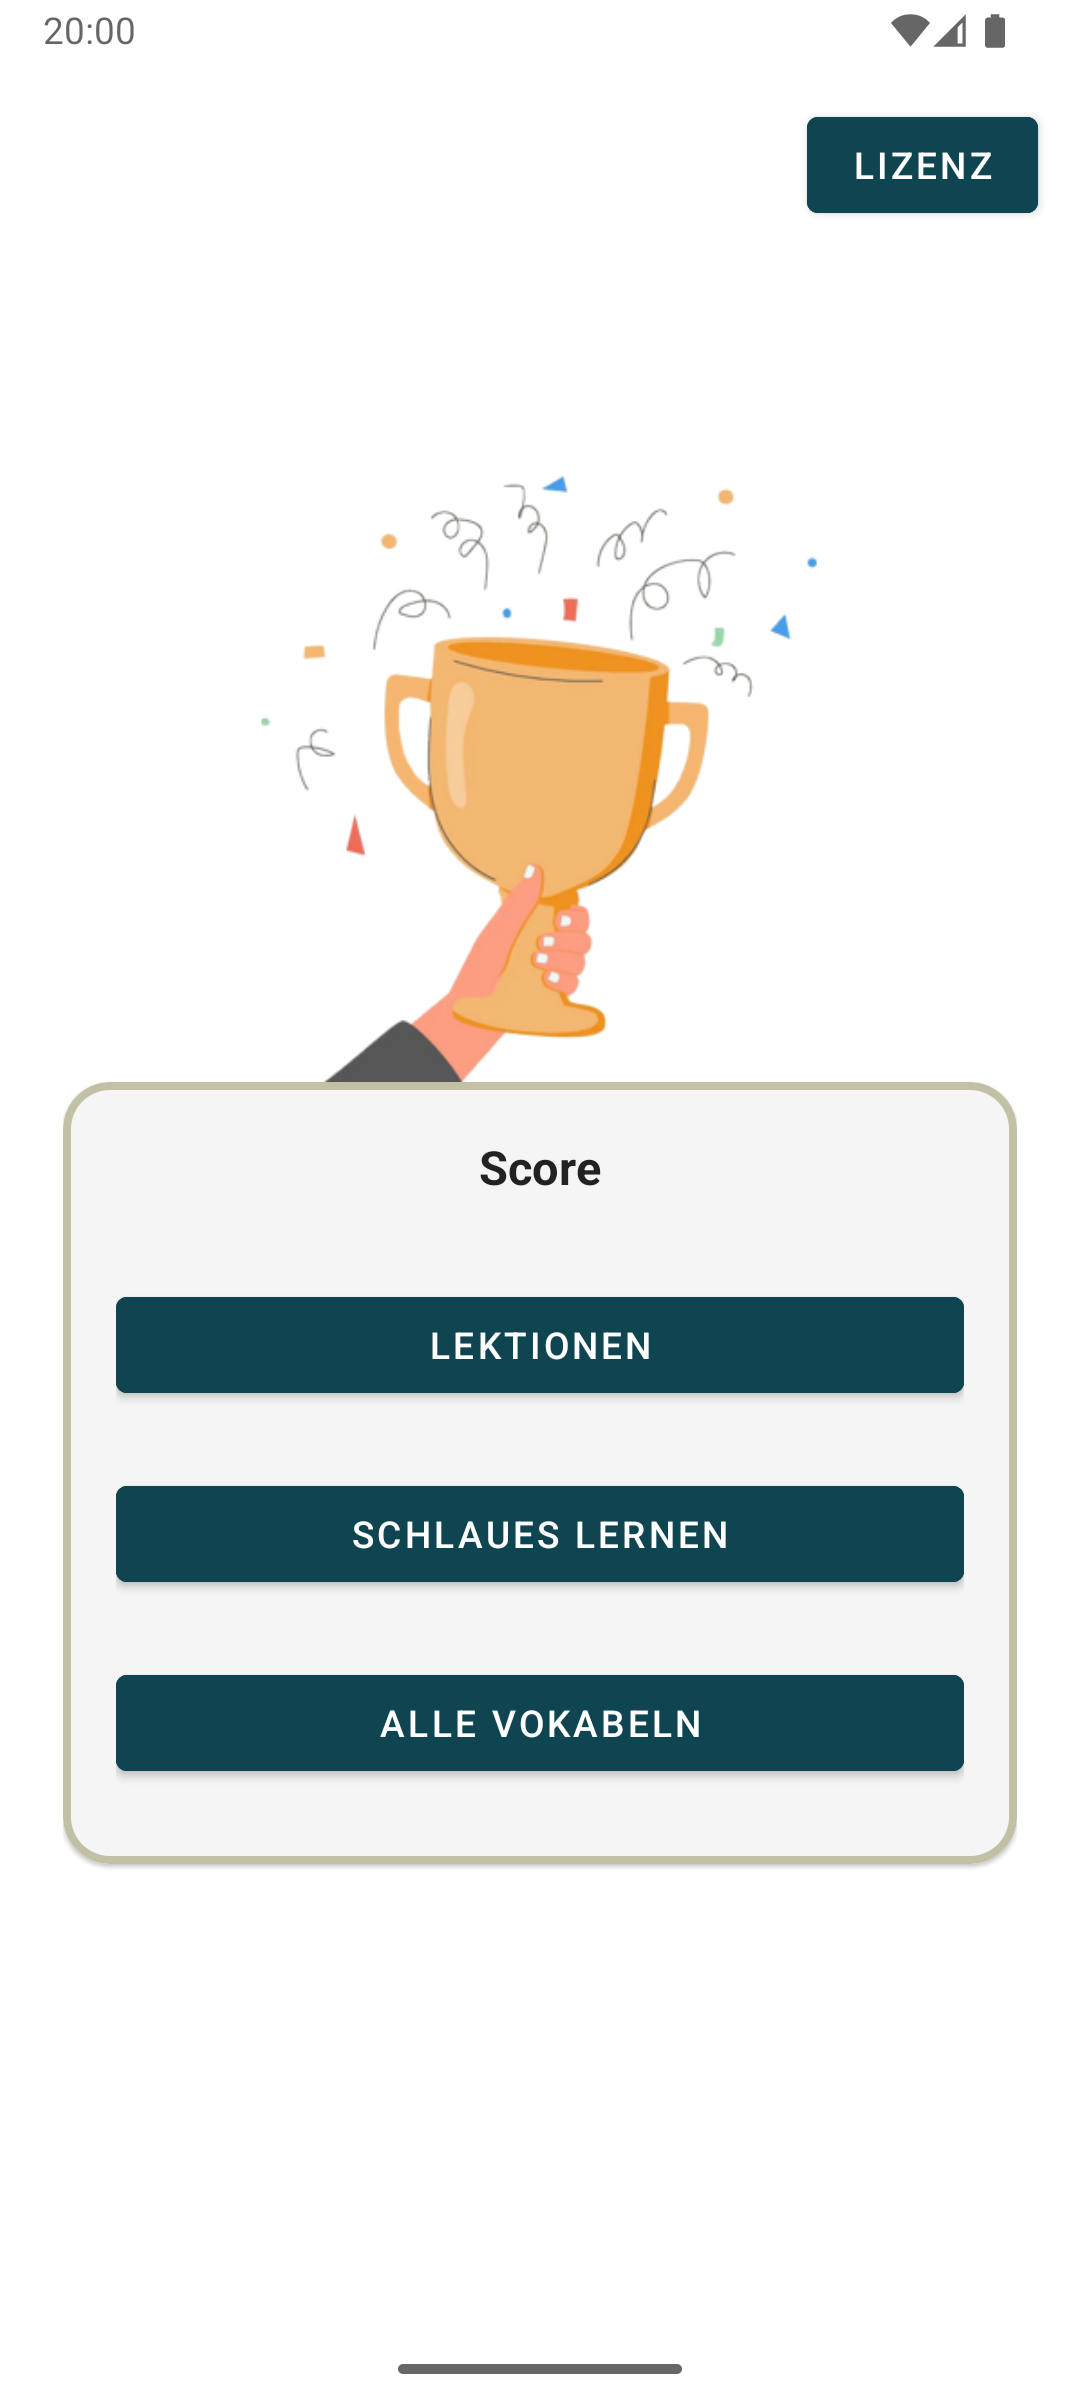
\includegraphics[width=\linewidth]{showcase/light_home.png}}
    \end{subcaptionbox}
    \hfill
    \begin{subcaptionbox}{dark\_guess\label{fig:bild2}}[0.25\linewidth]
        {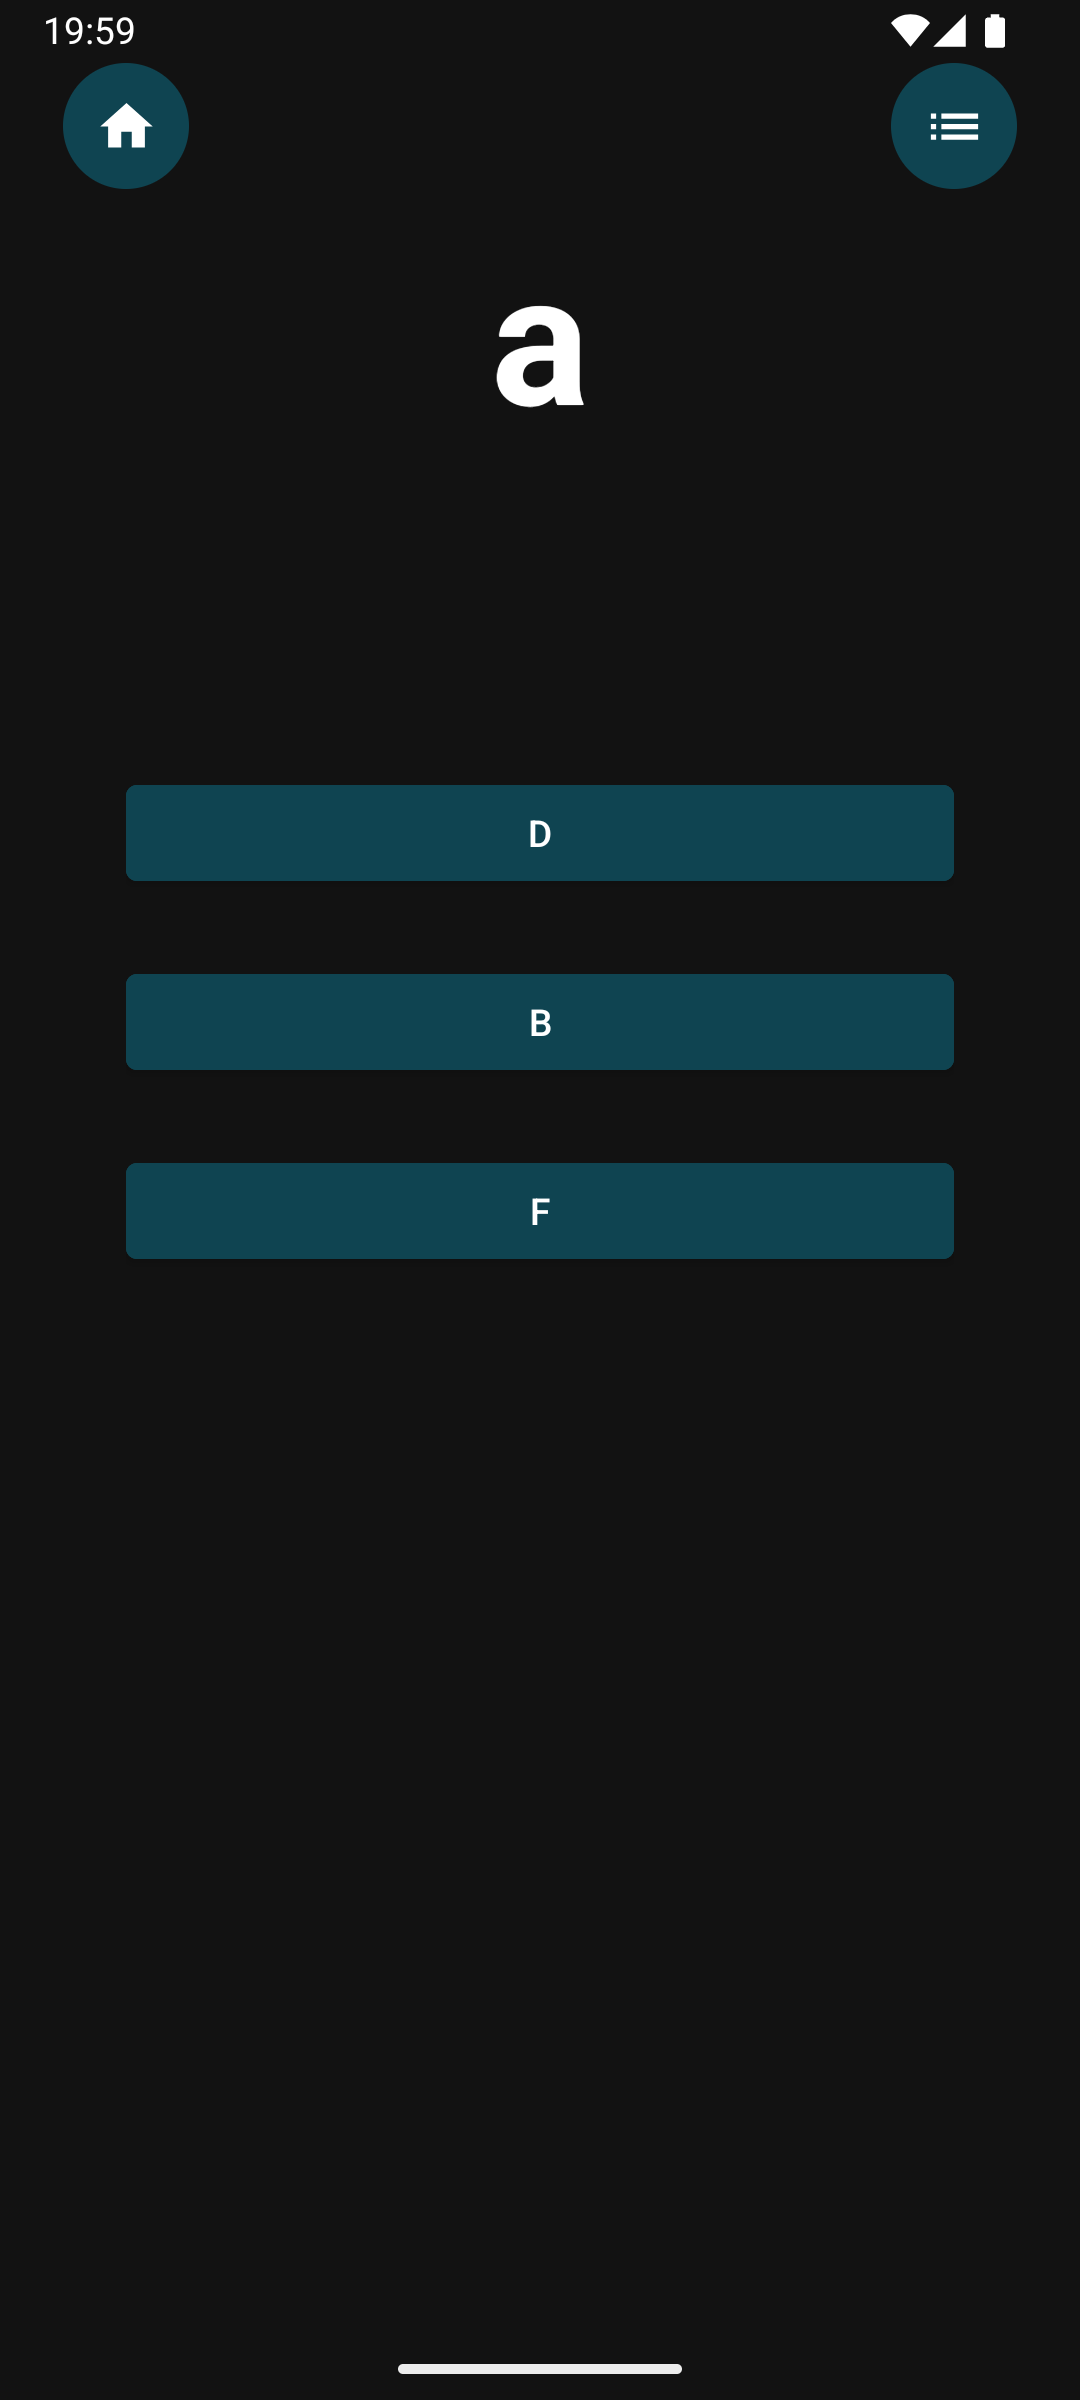
\includegraphics[width=\linewidth]{showcase/guess.png}}
    \end{subcaptionbox}
    \caption{Grundkonzept Home/Guess}
    \label{fig:nebeneinander}
\end{figure}

Befindet sich der Nutzer auf einer Unterseite, wie etwa bei der Vokabelabfrage oder innerhalb einer Lektion, kann er mittels der Android-Gestensteuerung zur vorherigen Seite zurückkehren. Oben links in der Ecke befindet sich zudem ein kleiner Button, der stets auf die Startseite führt. Dieser Button ist mit einem Haus-Symbol gekennzeichnet, das den Home-Bildschirm symbolisiert.

\begin{figure}[H]
    \centering
    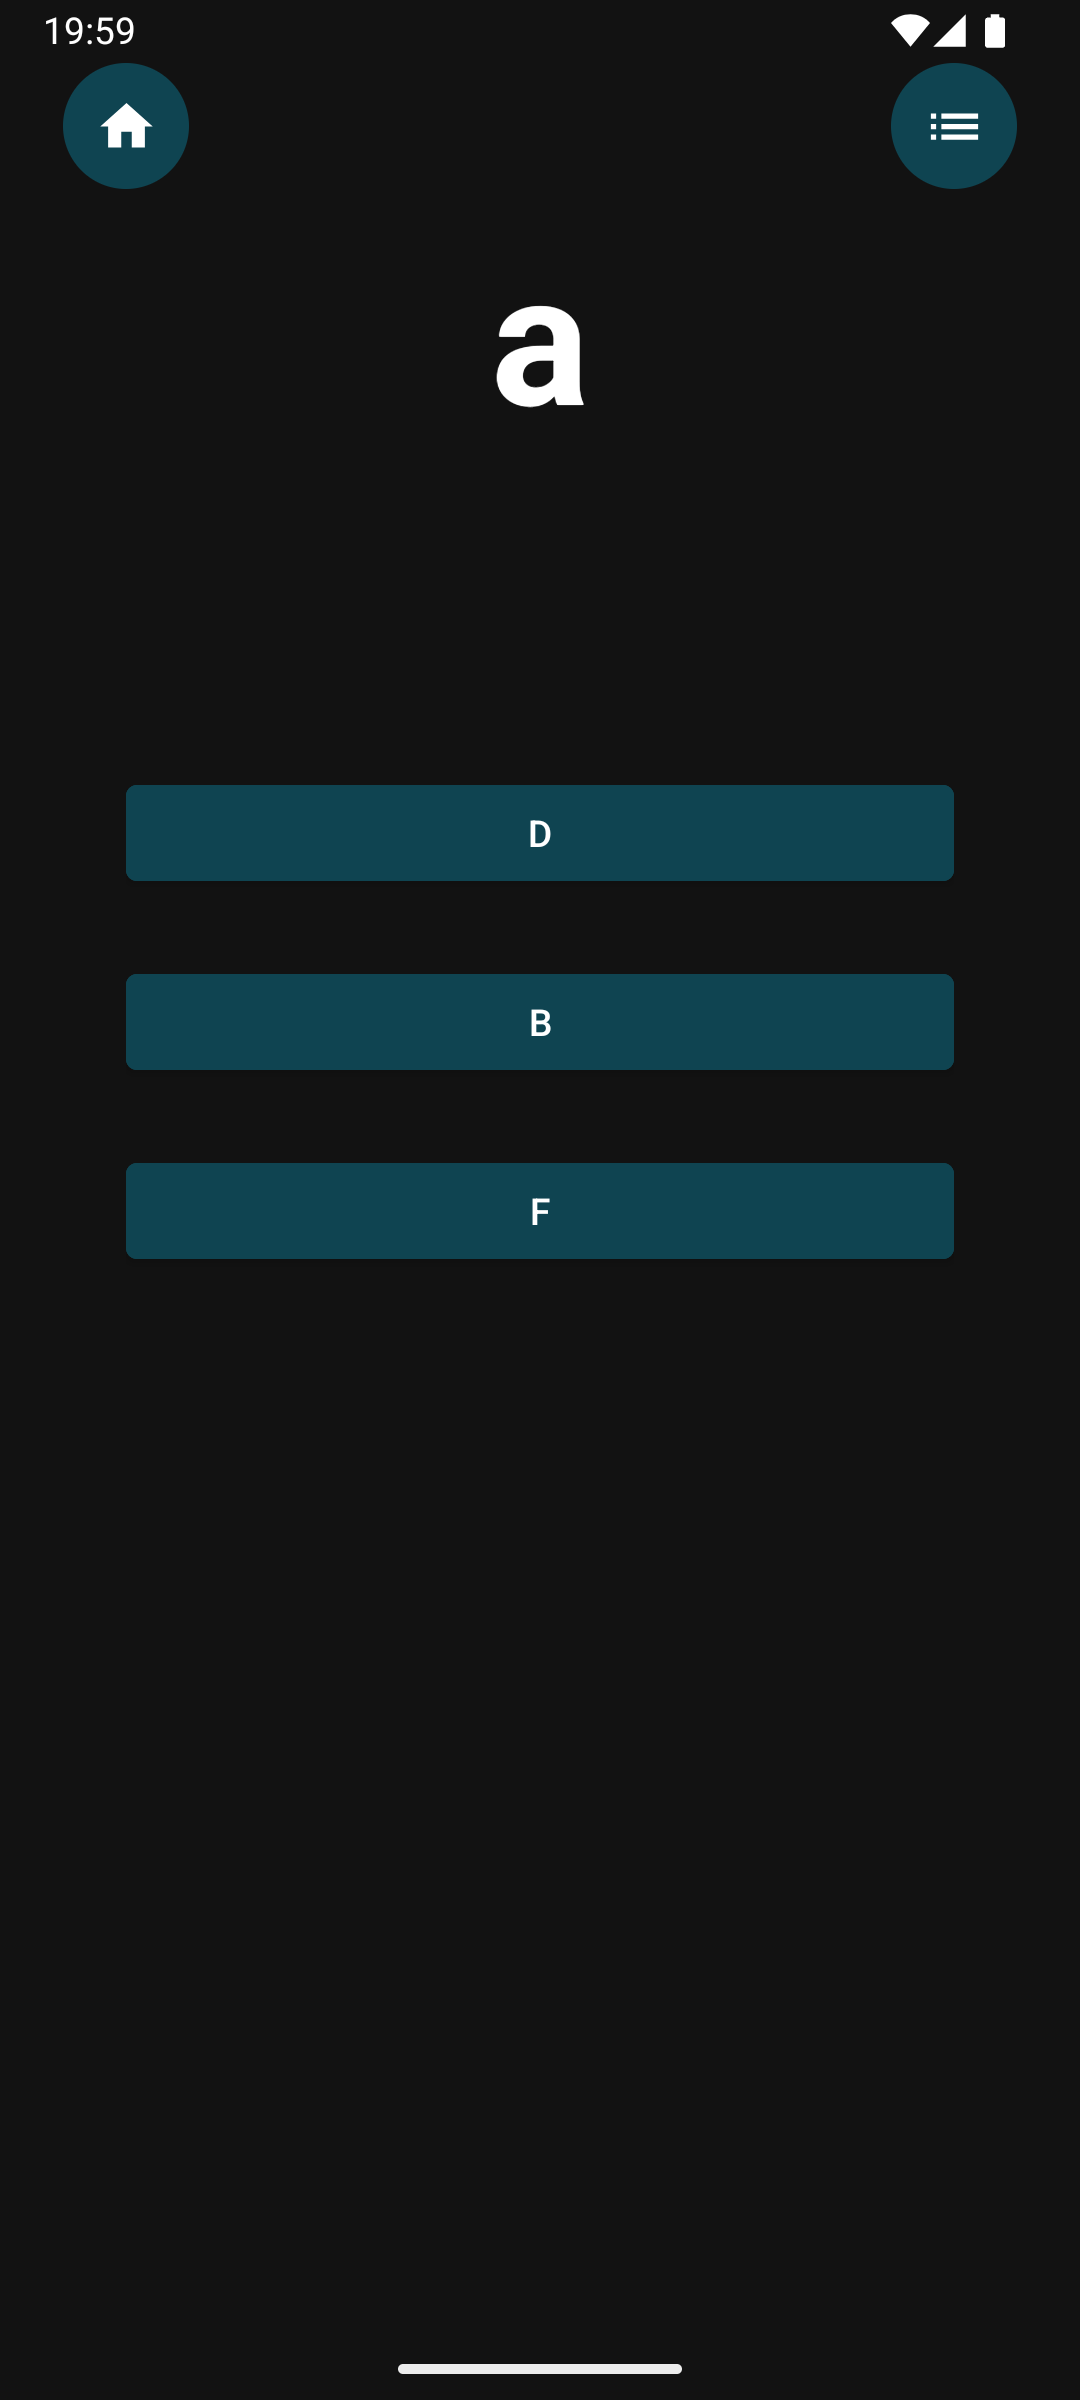
\includegraphics[width=0.4\textwidth]{showcase/guess.png}
    \caption{Lektionsabfrage – Beispiel}
    \label{fig:festes_bild}
\end{figure}

Der Button oben rechts führt zu einer Liste der Vokabeln, die aktuell abgefragt werden. Dieser Button ist mit einem Listen-Icon versehen.

\begin{figure}[H]
    \centering
    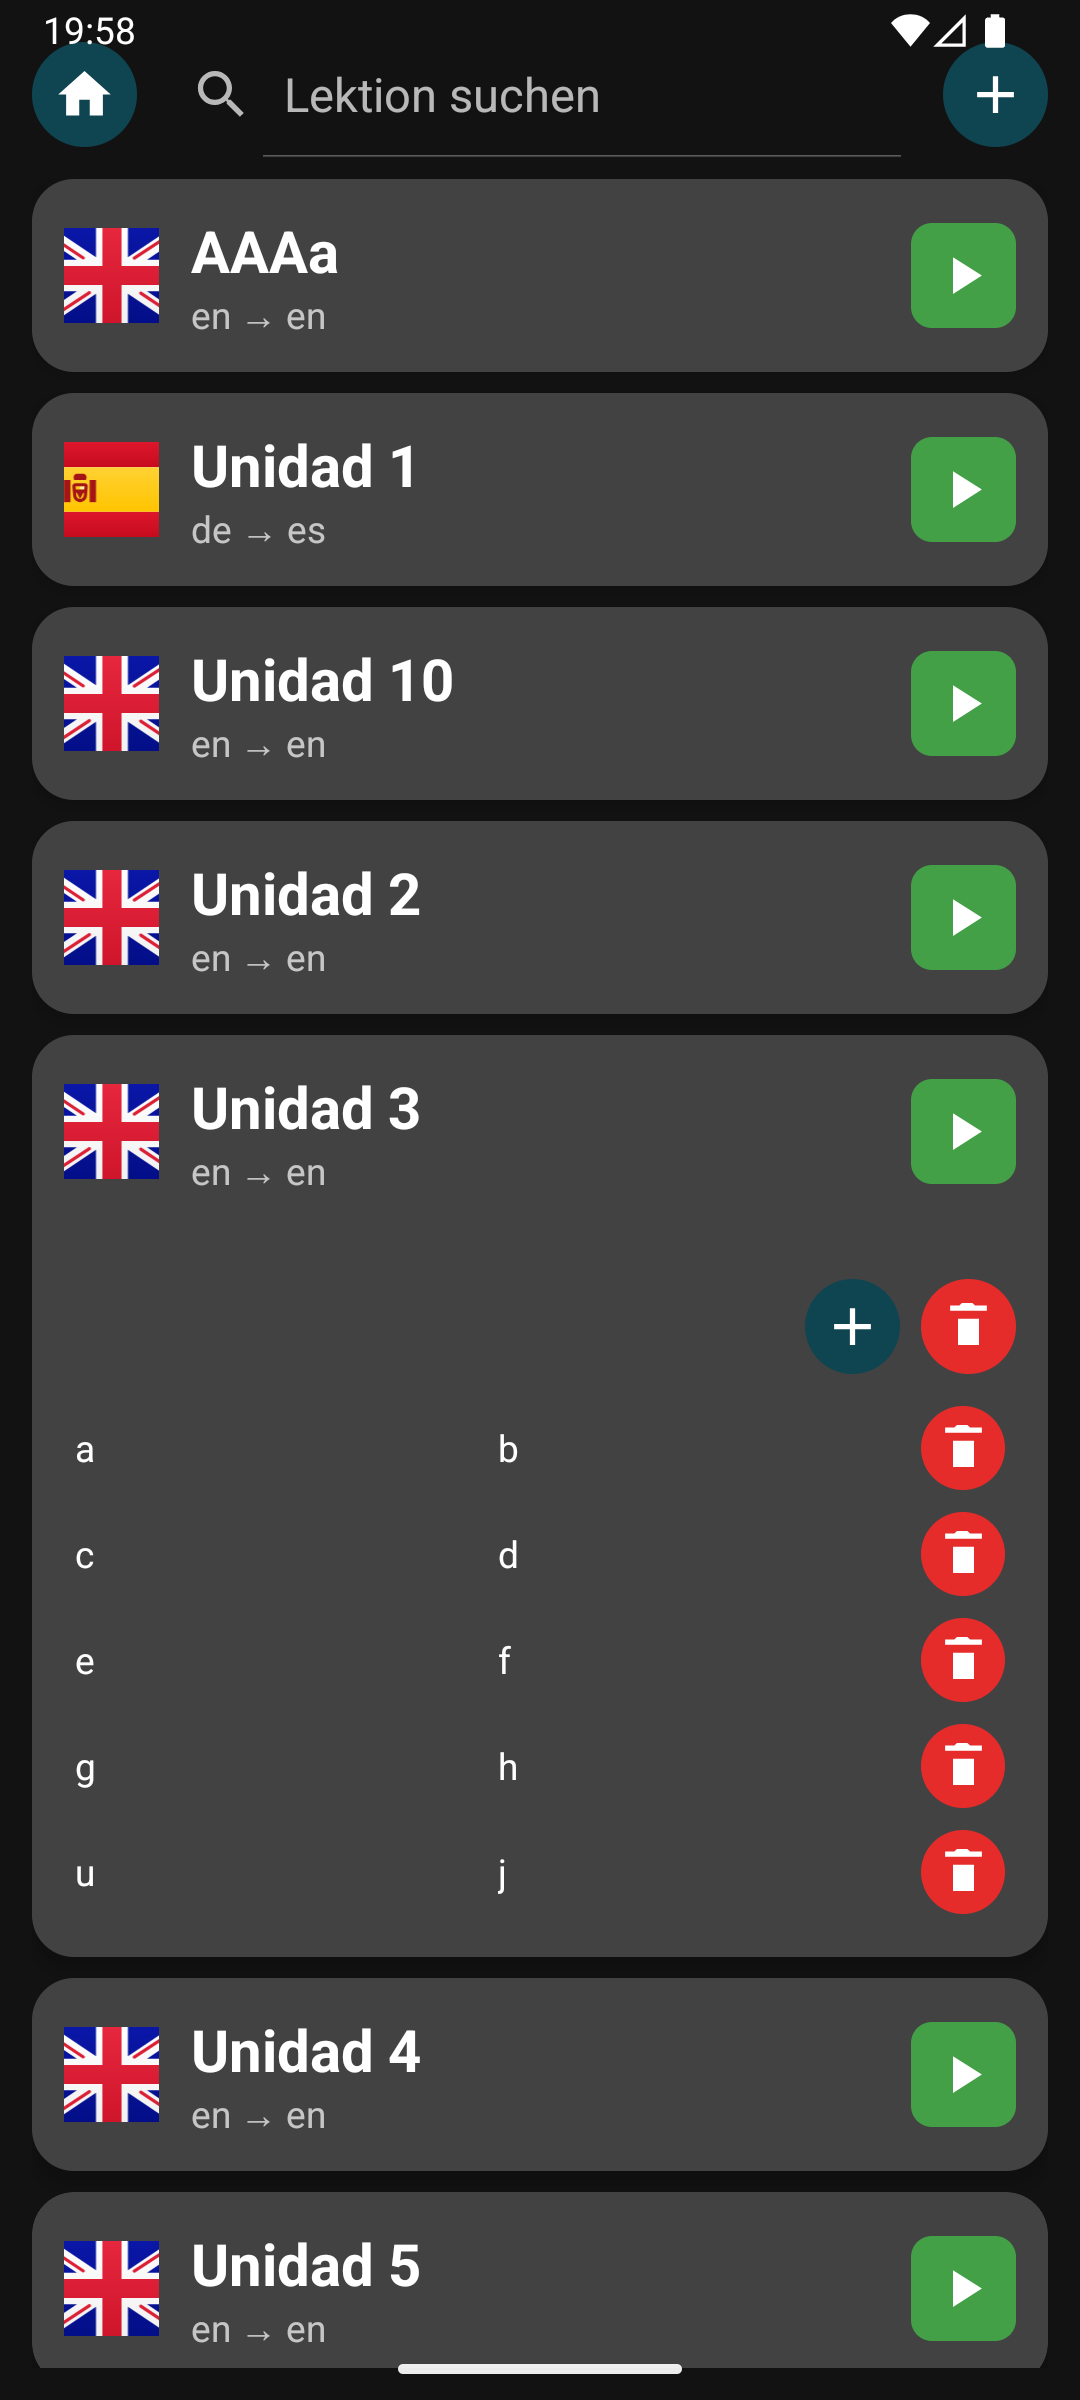
\includegraphics[width=0.4\textwidth]{showcase/Vokabeln.png}
    \caption{Vokabelliste – Beispiel}
    \label{fig:festes_bild}
\end{figure}

Buttons zum Löschen von Vokabeln oder Lektionen sind rot und mit einem Mülleimer-Icon gekennzeichnet. Alle Icons dienen dazu, ein schnelles Verständnis zu ermöglichen, welche Funktion die jeweiligen Buttons haben und wohin sie führen. Die Signalfarben unterstützen dabei, da sie das Bestätigen oder Löschen von Elementen verdeutlichen.

\newpage
\subsubsection*{Weitere Beispiele}

\begin{figure}[h]
    \centering
    \begin{subcaptionbox}{Lizenz\label{fig:bild1}}[0.2\linewidth]
        {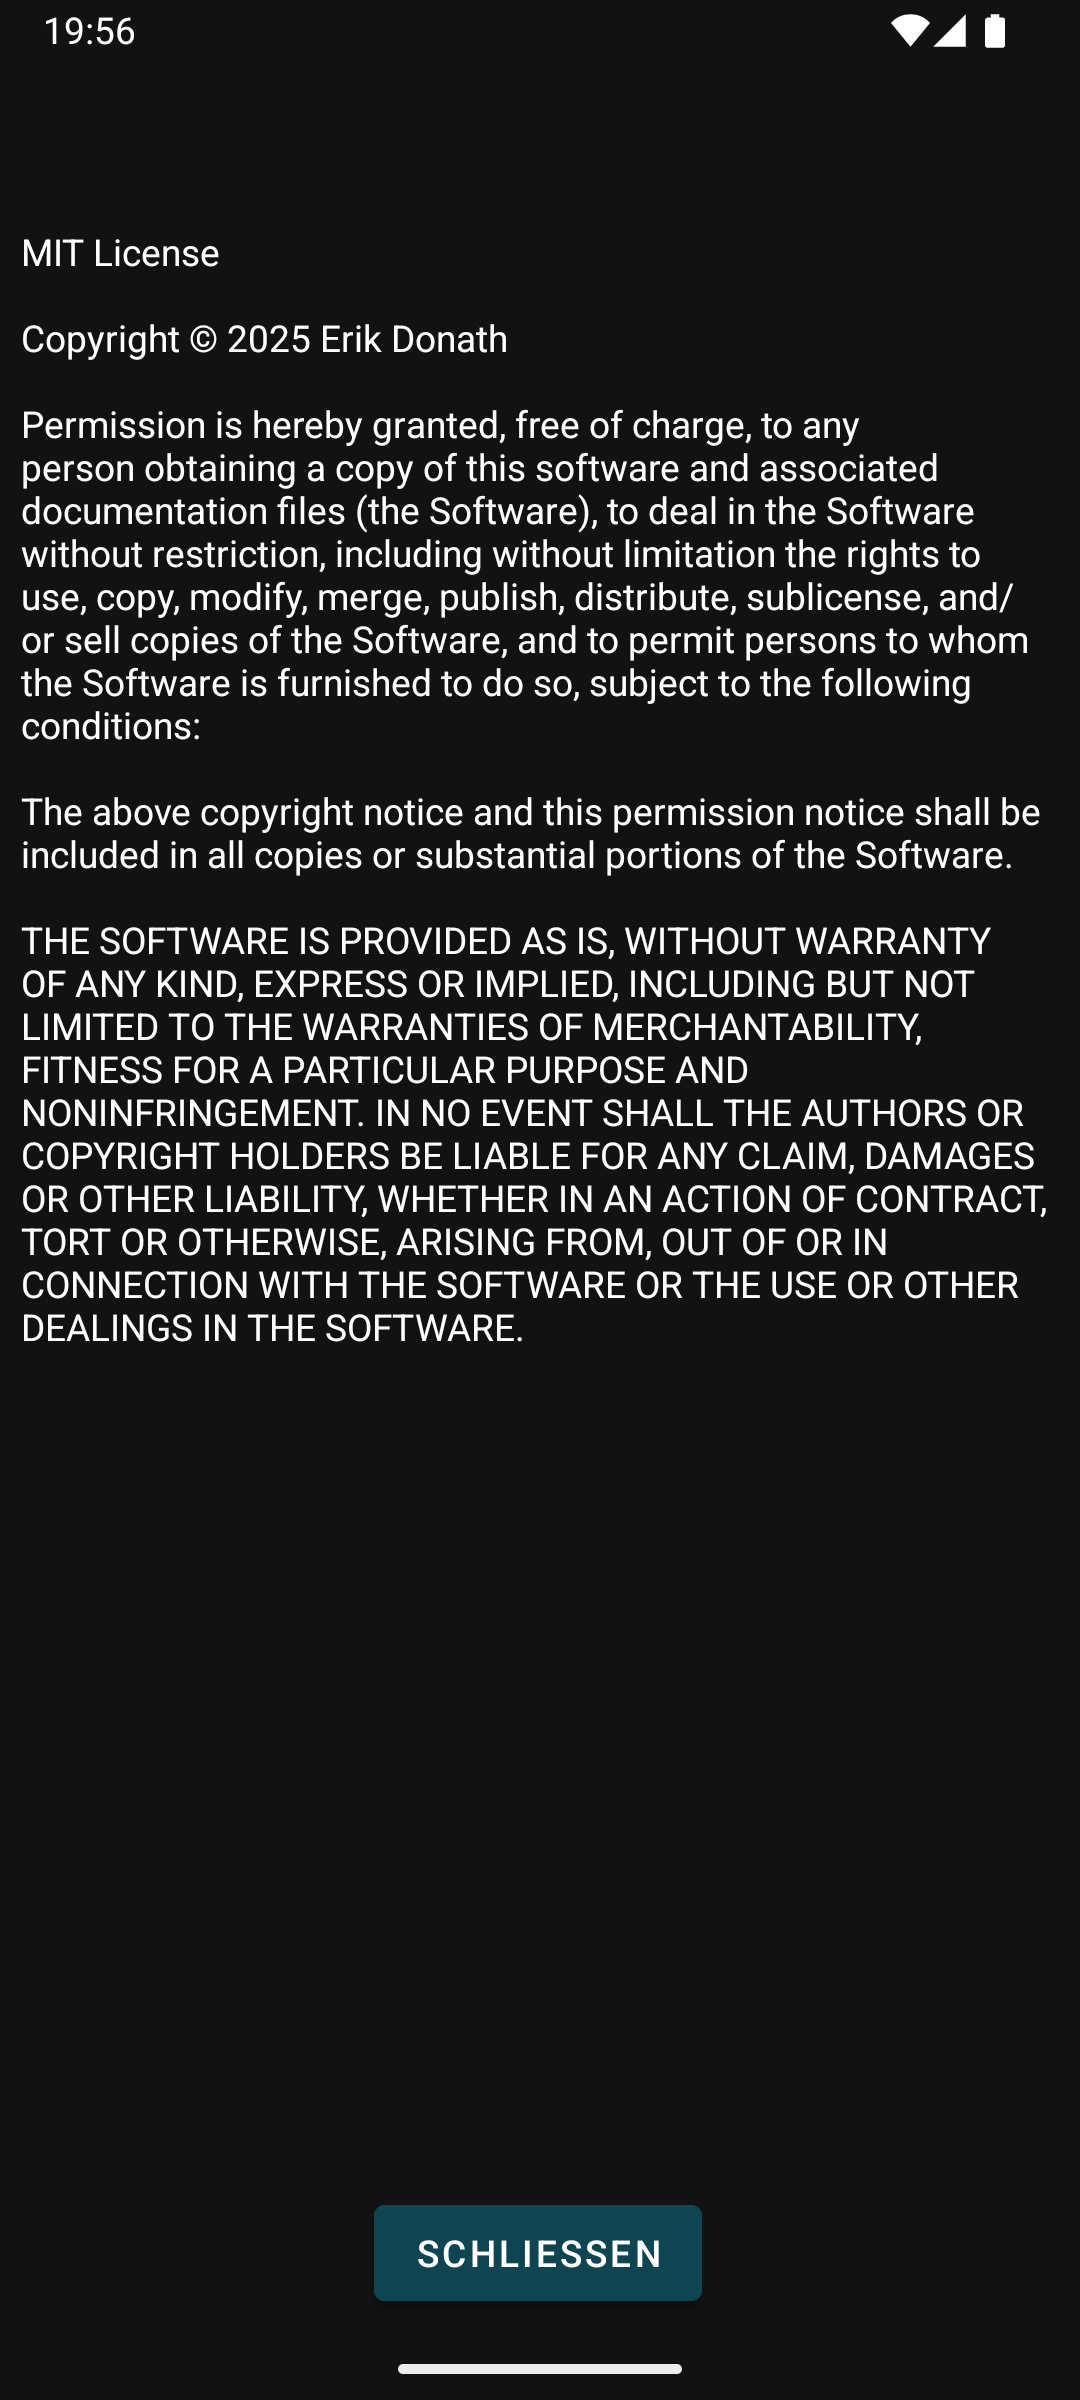
\includegraphics[width=\linewidth]{showcase/License.png}}
    \end{subcaptionbox}
    \hfill
    \begin{subcaptionbox}{Guess\label{fig:bild2}}[0.2\linewidth]
        {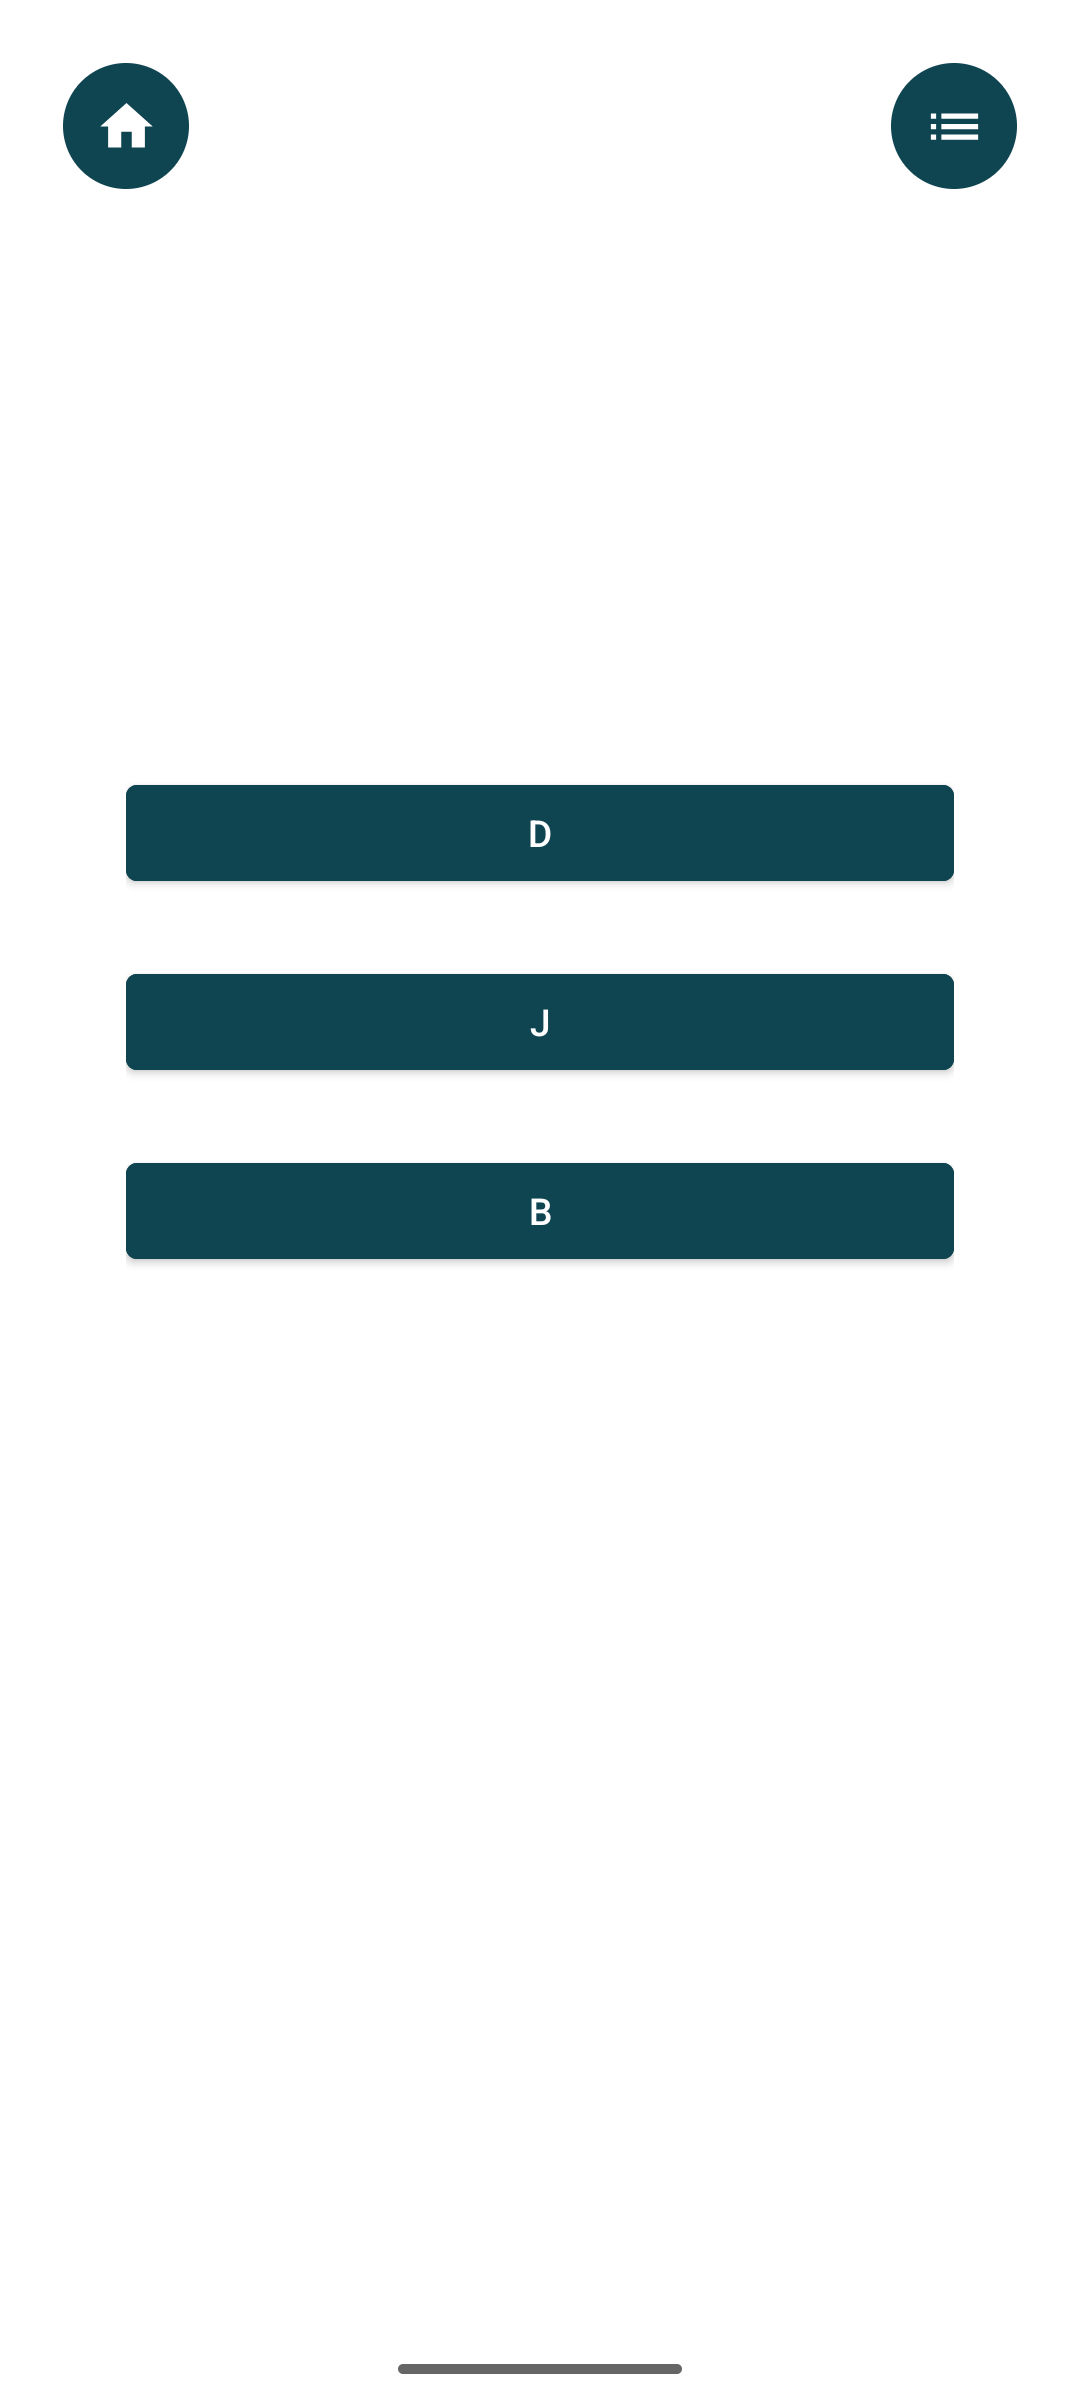
\includegraphics[width=\linewidth]{showcase/light_guess.png}}
    \end{subcaptionbox}
    \label{fig:nebeneinander}

    \centering
    \begin{subcaptionbox}{Ergebnis\label{fig:bild1}}[0.2\linewidth]
        {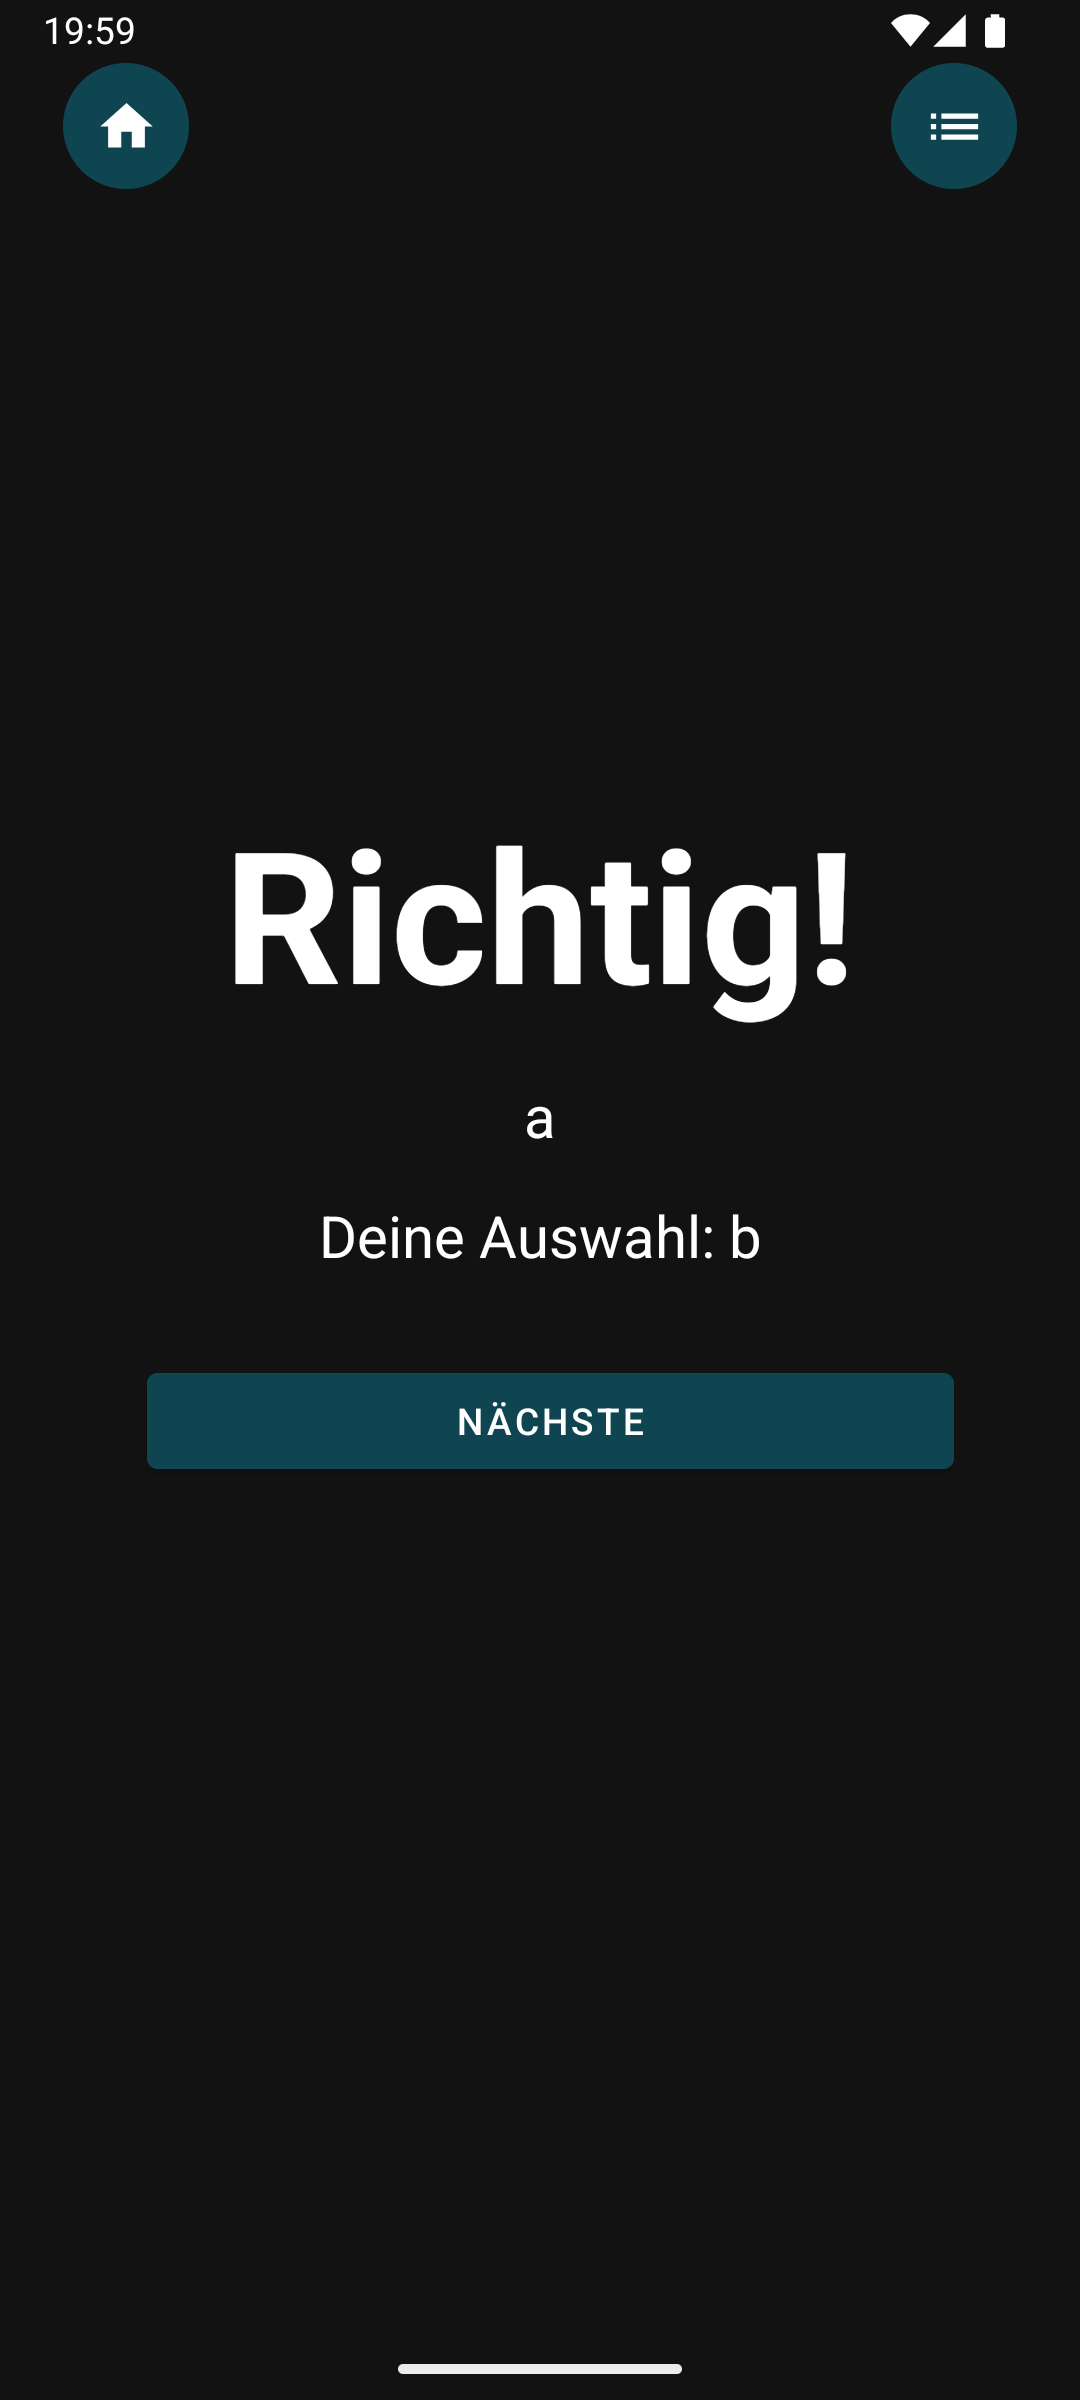
\includegraphics[width=\linewidth]{showcase/result.png}}
    \end{subcaptionbox}
    \hfill
    \begin{subcaptionbox}{Lektion hinzufügen\label{fig:bild2}}[0.2\linewidth]
        {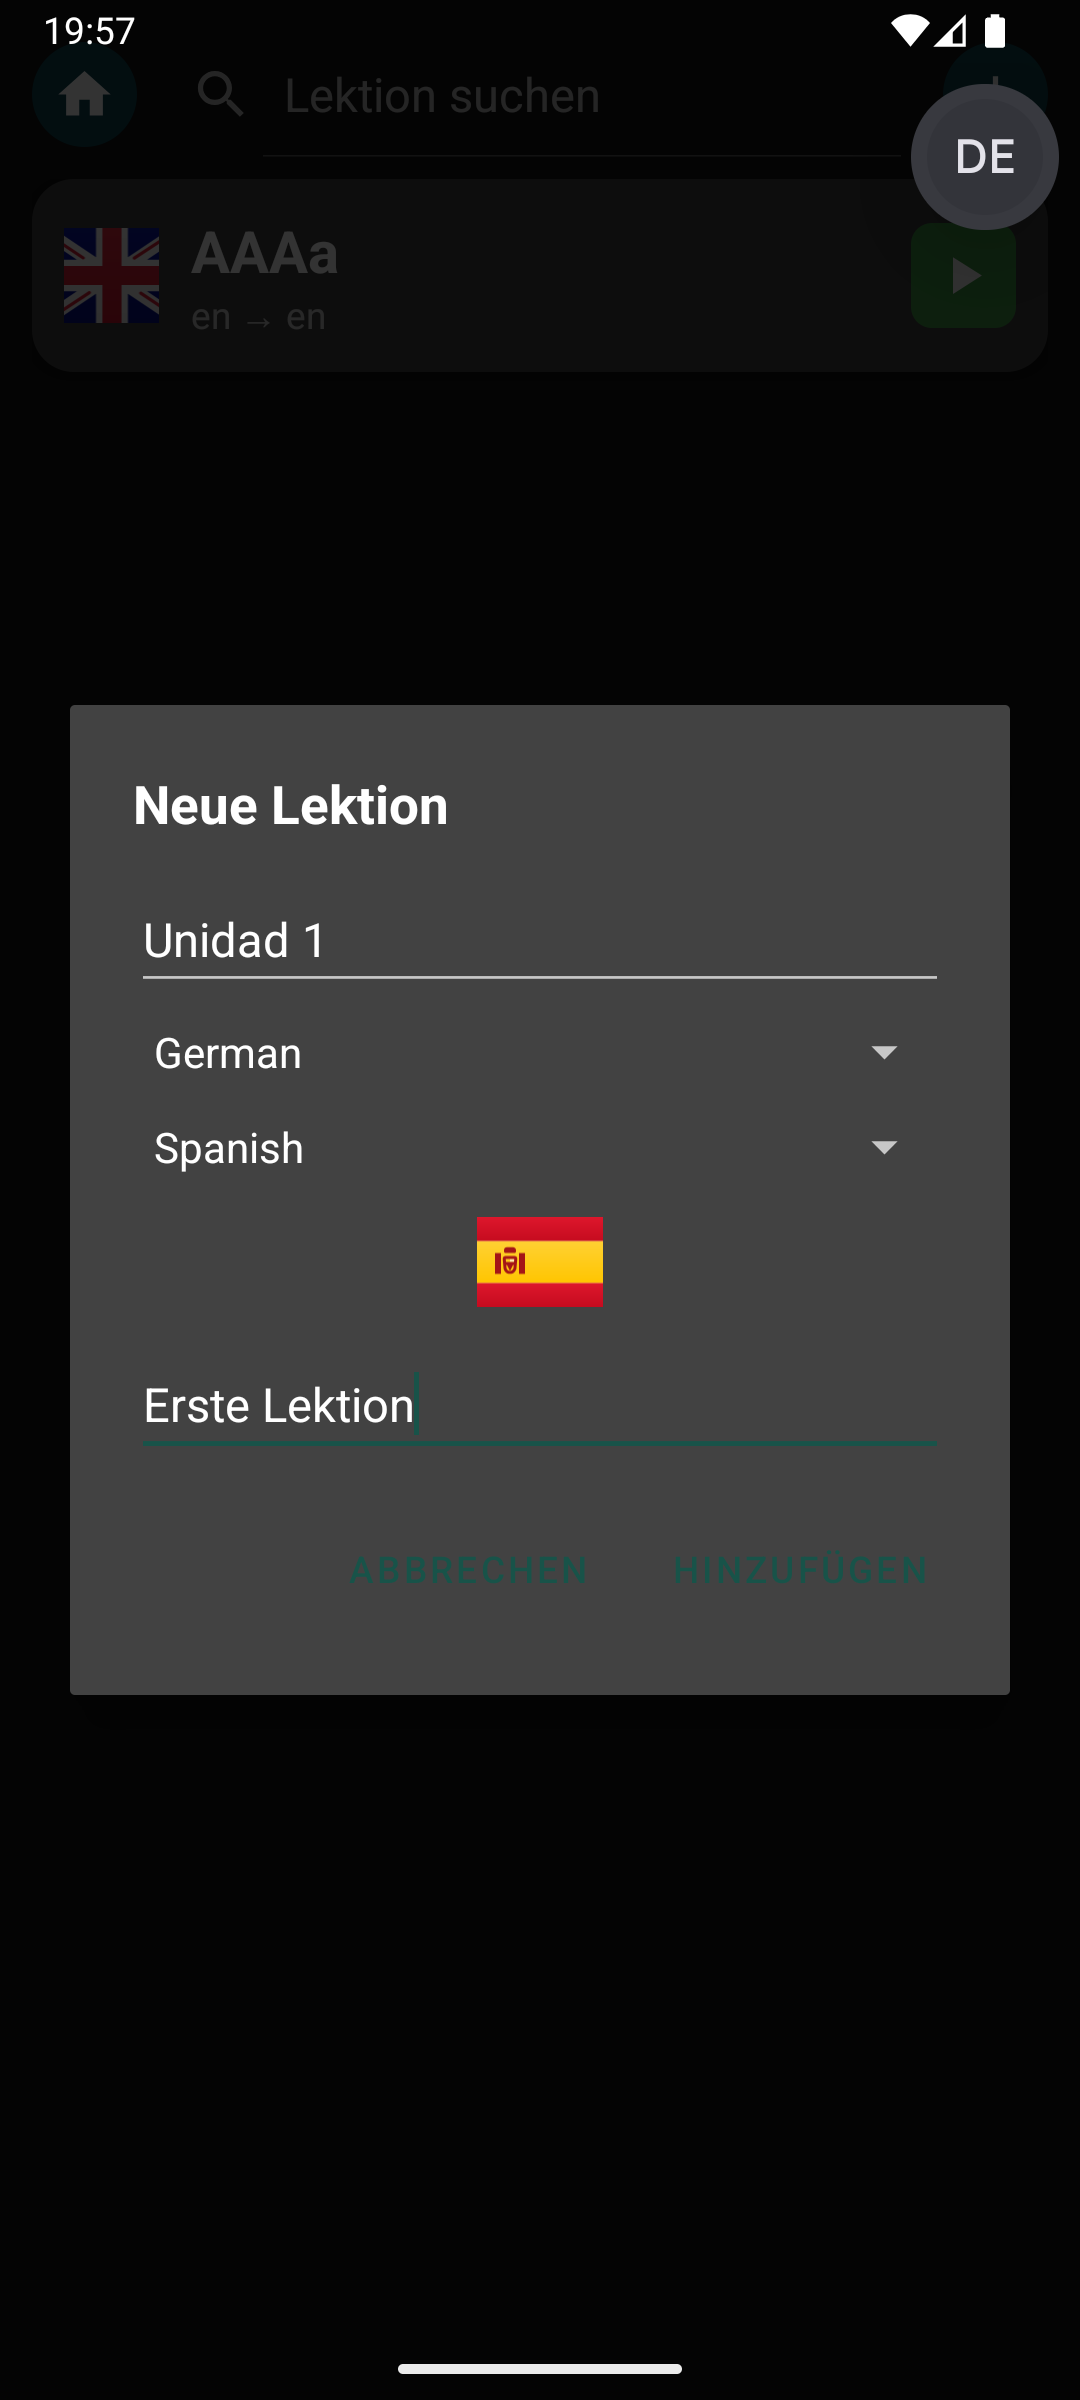
\includegraphics[width=\linewidth]{showcase/Add_Lektion.png}}
    \end{subcaptionbox}
    \caption{Weitere Beispiele}
    \label{fig:nebeneinander}
\end{figure}

\subsection{Datenmodelle}
\begin{figure}[H]
    \centering
    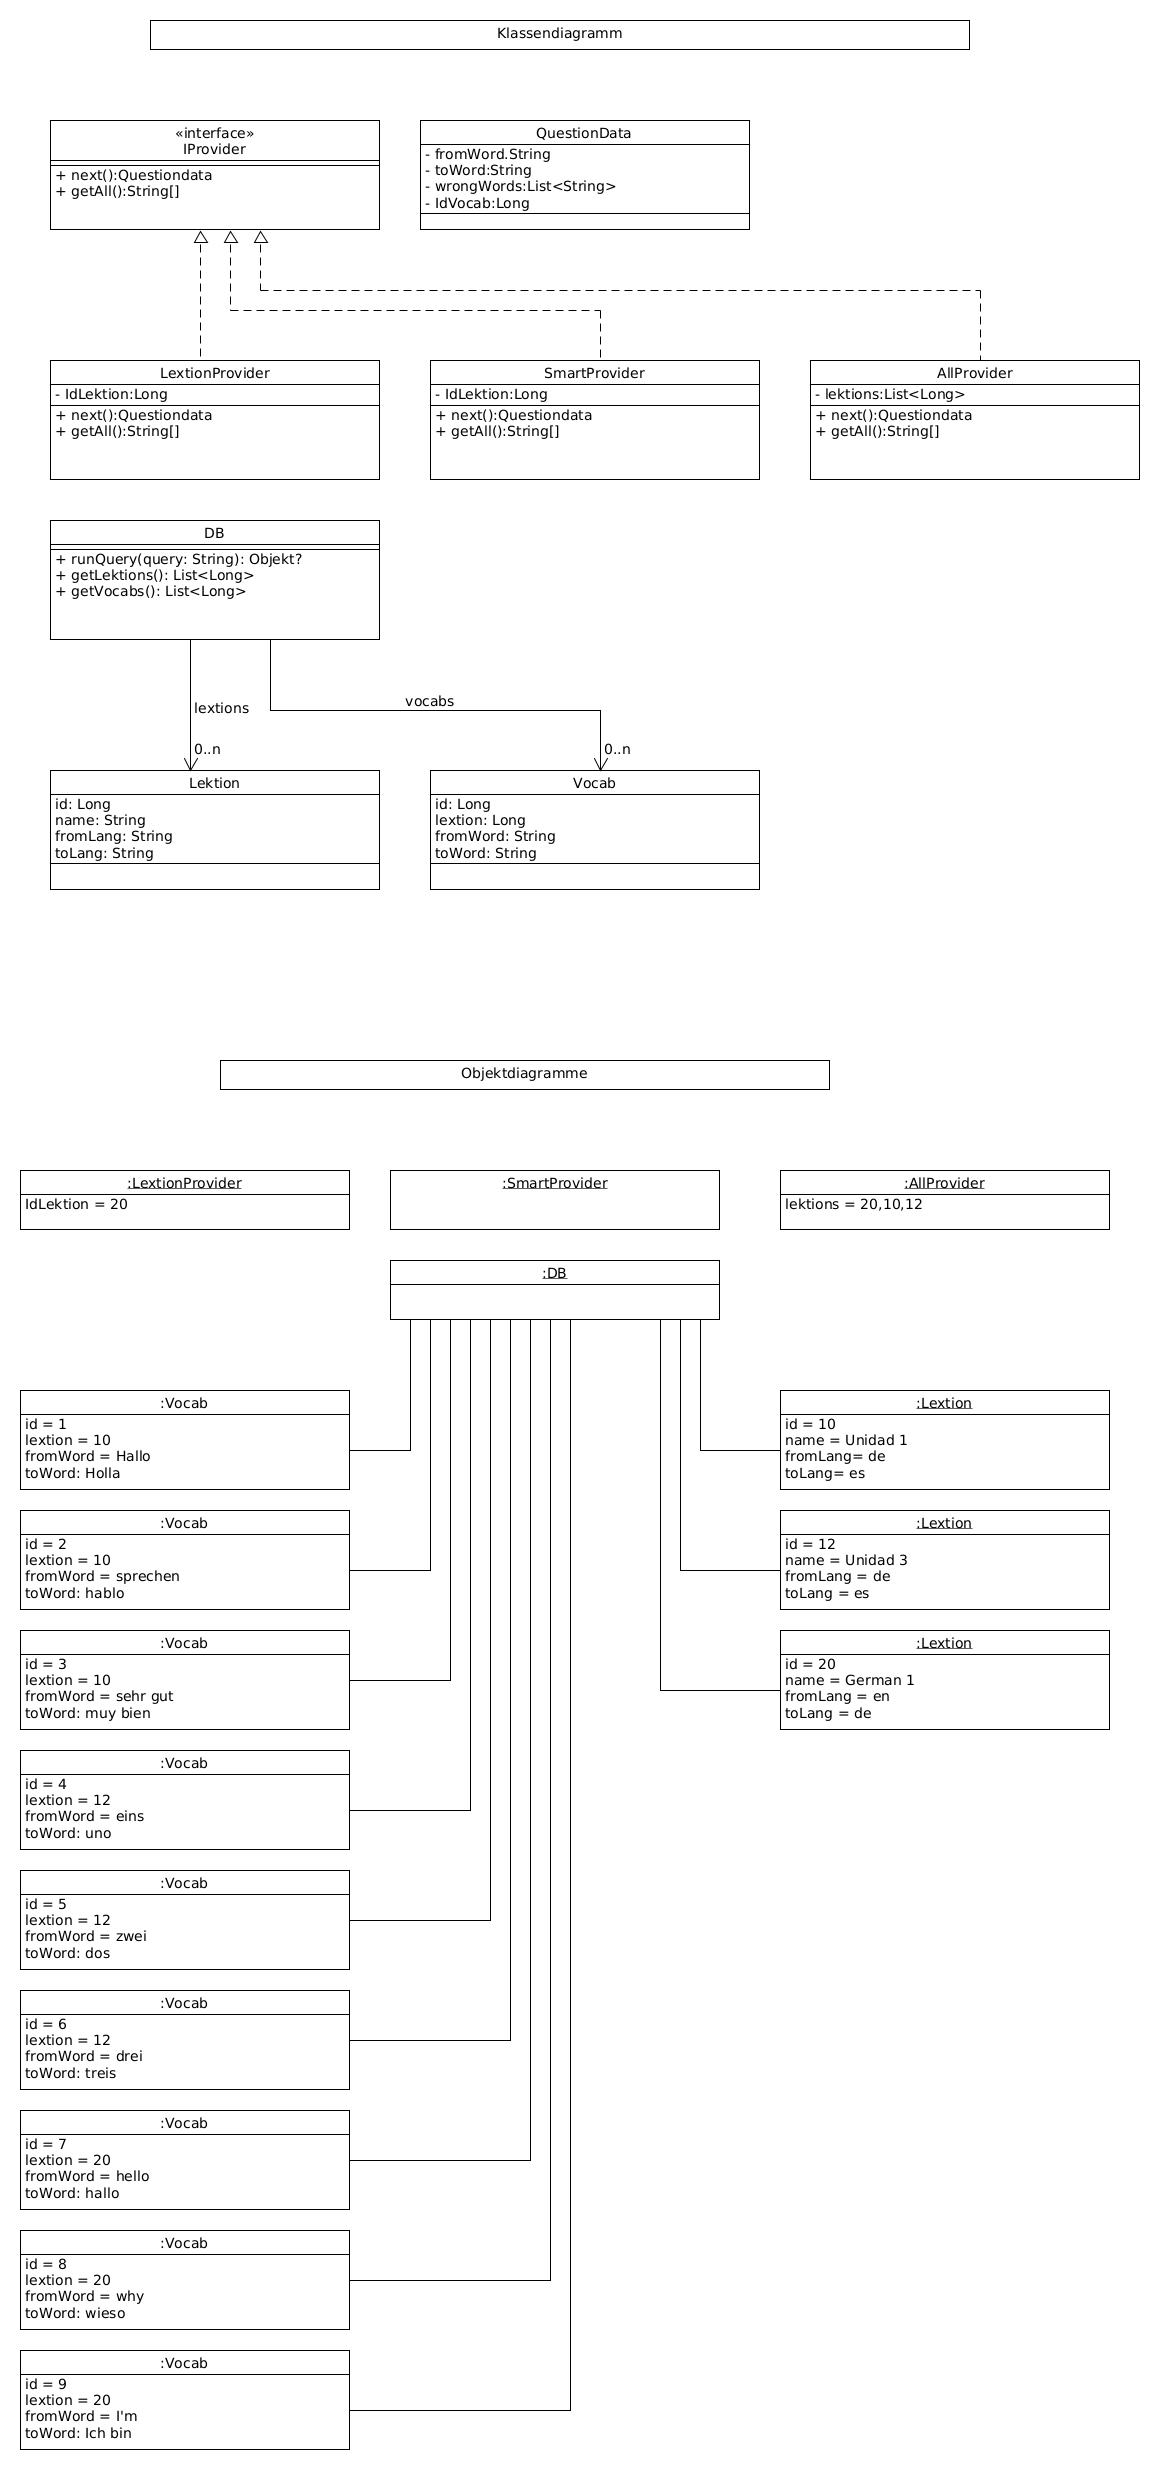
\includegraphics[width=0.7\textwidth]{Objekt-und Klassendiagramme-Erik,Daniel,Marit.jpg}
    \caption{Klassen und Objektdiagramm}
    \label{fig:festes_bild}
\end{figure}

\begin{figure}[H]
    \centering
    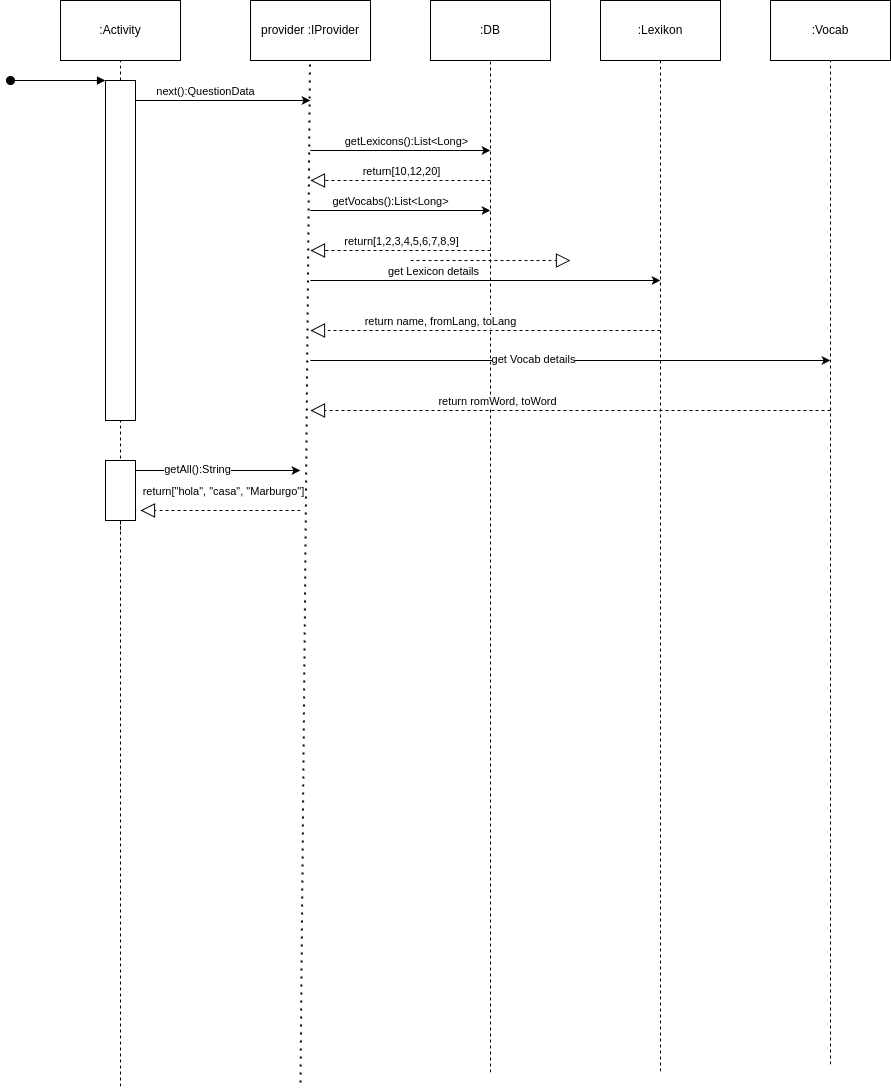
\includegraphics[width=0.7\textwidth]{sequenzdiagramm.png}
    \caption{Sequenzdiagramm}
    \label{fig:festes_bild}
\end{figure}

\section{Implementierung}

\subsection{Beschreibung des Vorgehens}
Die Implementierung erfolgte schrittweise mit Android Studio und Kotlin. Die Entwicklung war modular aufgebaut, um eine klare Trennung zwischen Benutzeroberfläche und Datenmanagement zu gewährleisten. Kernfunktionen wurden iterativ entwickelt und durch regelmäßige Commits im GitHub-Repository dokumentiert.

Zu Beginn wurde die Projektarchitektur eingerichtet und die Room-Datenbankbibliothek integriert. Parallel wurde die Benutzeroberfläche gestaltet und kontinuierlich verbessert, u.a. durch Dark Mode und Sprachunterstützung.

\subsubsection{Implementierung der Benutzeroberfläche}
Die Benutzeroberfläche wurde mit XML-Layouts in Android Studio erstellt und in Kotlin-Klassen eingebunden. Das MVVM-Muster trennte UI-Komponenten von der Logik. Die ursprüngliche Intent-basierte Navigation wurde durch ViewModels ersetzt, was die Zustandsverwaltung und Wiederverwendbarkeit verbesserte.

Das Design umfasste die Hauptaktivitäten, Anpassungen an verschiedene Darstellungsmodi (z.B. Dark Mode) und die Implementierung von UI-Elementen wie Buttons, Dialogen und Flaggen.

\subsubsection{Implementierung der Datenbank}
Zur Speicherung der Vokabeln und Lektionen wurde die Room-Datenbank verwendet. Die Datenbankstruktur wurde mehrfach überarbeitet, um Konsistenz und Erweiterbarkeit zu gewährleisten.

Provider-Klassen wie \texttt{AllProvider} und \texttt{LektionProvider} kapseln den Datenbankzugriff und stellen die Daten für die UI bereit. Fehlerfälle bei fehlenden Vokabeln werden behandelt.

\subsection{Umfang des Quellcodes}

Um einen Überblick über die technische Dimension des Projekts zu geben, werden im Folgenden die wesentlichen Kennzahlen zur Codebasis dargestellt. Die Angabe der Codezeilen und Dateitypen hilft, den Umfang und die Komplexität der Entwicklung einzuschätzen und erleichtert künftigen Entwickler:innen die Orientierung im Projekt.

Die folgende Tabelle zeigt die wichtigsten Bestandteile des Quellcodes sowie deren Umfang zum Zeitpunkt der Abgabe:

\begin{table}[H]
\centering
\caption{Überblick über die wichtigsten Projektdateien und Codezeilen}
\begin{tabular}{lrr}
\toprule
\textbf{Dateityp} & \textbf{Dateien} & \textbf{Codezeilen} \\
\midrule
Kotlin    & 25  & 773 \\
XML       & 88  & 5\,036 \\
JSON      & 2   & 152 \\
Markdown  & 1   & 46 \\
TeX       & 1   & 206 \\
\midrule
\textbf{Summe}   & \textbf{117} & \textbf{6\,213} \\
\bottomrule
\end{tabular}
\end{table}

Die größte Codebasis entfällt auf die XML-Dateien, in denen die Benutzeroberfläche und Layouts definiert sind. Der Kern der Anwendungslogik ist in Kotlin implementiert. Hinzu kommen Konfigurations- und Dokumentationsdateien in JSON, Markdown und TeX.

Eine detaillierte Aufschlüsselung aller weiteren Dateitypen und deren Umfang befindet sich im Anhang.

\section{Schlussfolgerung und Ausblick}

\subsection{Soll-Ist-Vergleich}
Alle im Abschnitt \textit{Soll-Analyse} definierten Funktionen wurden wie geplant umgesetzt. Ein Vergleich zwischen Soll und Ist ist daher nicht erforderlich.

\subsection{Begründung für Abweichungen}
Im Projektverlauf traten einige Abweichungen vom ursprünglichen Plan auf. Hauptgründe waren Zeitdruck in der Endphase, Koordinationsprobleme im Team und technische Herausforderungen bei Wunschfunktionen wie dem Punktesystem oder der iOS-Portierung. Einige Wunschkriterien wurden zugunsten der Kernfunktionen zurückgestellt. Die Dokumentation wurde nicht immer zeitnah gepflegt, was die Nachvollziehbarkeit erschwerte.

\subsection{Fazit und Ausblick}
Das Projekt „Palabra“ hat im Rahmen der Gruppenarbeit zahlreiche Erkenntnisse sowohl hinsichtlich der Strukturierung als auch der Zusammenarbeit im Team hervorgebracht. Zu Beginn wurde eine Tabelle zur Dokumentation von Problemen eingerichtet, um deren Entwicklung nachvollziehen zu können. Leider wurde diese gegen Ende des Projekts nicht mehr konsequent genutzt, sodass die Nachvollziehbarkeit einzelner Problemstellungen im Rückblick erschwert wurde. Trotz festgelegter Termine konnten einige Abgaben nicht rechtzeitig fertiggestellt werden, was insbesondere bei der Erstellung und Nutzung von Diagrammen zu Zeitdruck führte. Eine der größten Herausforderungen bestand darin, das Team regelmäßig zusammenzubringen und gemeinsam an den zugewiesenen Aufgaben zu arbeiten. Obwohl der grundsätzliche Aufbau des Projekts zu Beginn klar war, wurde es mit fortschreitender Entwicklung zunehmend schwieriger, den Überblick über fehlende Elemente und offene Aufgaben zu behalten.

Auch die Arbeit am Code gestaltete sich phasenweise ernüchternd. Zwar war von Anfang an festgelegt, dass die Entwicklung in Android Studio erfolgen sollte, dennoch wurde diese Entscheidung gegen Ende des Projekts hinterfragt – insbesondere im Hinblick auf alternative Entwicklungsumgebungen oder Programmiersprachen, die beispielsweise eine einfachere Datenbankanbindung ermöglicht hätten. Letztlich blieb es jedoch bei der ursprünglichen Wahl, auch wenn diese Überlegungen kurzzeitig für Unsicherheit sorgten.

Die Dokumentation stellte ein weiteres Problemfeld dar. Aufgrund unklarer Strukturen, häufiger Umstrukturierungen und zeitweiliger Vernachlässigung war die Dokumentation nicht immer auf dem aktuellen Stand. Rückblickend wurde deutlich, dass insbesondere die kontinuierliche Pflege der Dokumentation und die frühzeitige Fertigstellung von unterstützenden Materialien wie Diagrammen entscheidend für einen reibungslosen Projektverlauf sind.

Positiv hervorzuheben ist die von Beginn an funktionierende Versionskontrolle über GitHub. Die konsequente Nutzung dieses Tools hat dazu beigetragen, viele Probleme frühzeitig zu erkennen und nachzuvollziehen. Die Versionskontrolle wird auf jeden Fall auch in zukünftigen Projekten einen festen Platz einnehmen.

Ein weiteres wichtiges Lernfeld war der Umgang mit auftretenden Problemen. Es hat sich gezeigt, dass deren Dokumentation und Nachverfolgung nicht vernachlässigt werden dürfen. Für künftige Projekte wäre es sinnvoll, eine standardisierte Vorlage für die Problemdokumentation zu entwickeln, an der sich alle Teammitglieder orientieren können. Dabei ist zu beachten, dass nicht alle Probleme zwangsläufig von den für die Dokumentation zuständigen Personen erfasst werden – hier bedarf es klarer Absprachen im Vorfeld.

Auch sollte zu Beginn eines Projekts verbindlich festgelegt werden, wie die technische Basis – insbesondere die Wahl der Programmiersprache und Entwicklungsumgebung – aussieht. Diese Entscheidungen sollten nicht erst gegen Ende des Projekts hinterfragt werden, sondern bereits in der Planungsphase gemeinsam recherchiert und abgestimmt werden.

Abschließend lässt sich festhalten, dass das Projekt trotz aller Herausforderungen und Schwierigkeiten ein zufriedenstellendes Ergebnis hervorgebracht hat. Die Motivation, künftig auch die Wunschkriterien zu realisieren, ist hoch. Die im Verlauf des Projekts aufgetretenen Probleme werden als wertvolle Erfahrungen betrachtet und dienen als Grundlage für Verbesserungen in zukünftigen Projekten. Insgesamt war das Projekt „Palabra“ ein lehrreicher Prozess, der sowohl die Stärken als auch die Optimierungspotenziale der Teamarbeit und Projektorganisation aufgezeigt hat.

\appendix

\section{Anhang}

Da der vollständige Quellcode mit 773 Zeilen in Kotlin und 5.036 Zeilen in XML sehr umfangreich ist, würde ein Abdruck im Anhang den Rahmen dieser Dokumentation sprengen. Aus diesem Grund wird an dieser Stelle auf das entsprechende GitHub-Repository verwiesen. Der folgende Link führt Sie zu dem Quellcode zum Zeitpunkt der Abgabe dieser Dokumentation:  
\href{https://github.com/Erik-Donath/Palabra/tree/cc55c524ebff2f6db85a36f6ec2c0afb23070e2f}{GitHub-Link zum Quellcode}.

\subsection*{Überblick über die Projektdateien}

Die folgende Tabelle gibt einen Überblick über die im Projekt enthaltenen Dateien und deren Umfang:

\begin{table}[htbp]
\centering
\caption{Überblick über die Projektdateien}
\begin{tabularx}{\textwidth}{lrrrr}
\toprule
\textbf{Sprache/Dateityp} & \textbf{Dateien} & \textbf{Leerzeilen} & \textbf{Kommentare} & \textbf{Codezeilen} \\
\midrule
XML            & 88  & 88  & 58  & 5\,036 \\
Kotlin         & 25  & 135 & 8   & 773    \\
TeX            & 1   & 67  & 0   & 206    \\
JSON           & 2   & 0   & 0   & 152    \\
Bourne Shell   & 1   & 23  & 36  & 126    \\
Gradle         & 3   & 16  & 8   & 104    \\
DOS Batch      & 1   & 21  & 2   & 66     \\
Markdown       & 1   & 25  & 0   & 46     \\
TOML           & 1   & 2   & 0   & 36     \\
Properties     & 4   & 0   & 28  & 11     \\
Text           & 1   & 0   & 0   & 1      \\
ProGuard       & 1   & 3   & 18  & 0      \\
\midrule
\textbf{Summe} & \textbf{129} & \textbf{380} & \textbf{158} & \textbf{6\,557} \\
\bottomrule
\end{tabularx}
\end{table}

\textit{Stand: Mittwoch, 28. Mai 2025, 20:00 Uhr (CEST)}
\\\\
Wobei zu bedenken ist, dass hierbei auch Skripte des Build-Systems sowie die Dokumentation selbst betrachtet werden. Die für die Bewertung relevanten Sprachen sind Kotlin, XML, JSON und ggf. Markdown sowie TeX.

\newpage
\subsection*{Verwendete Bilder und Grafiken}

Im Folgenden sind alle in der Dokumentation verwendeten Grafiken tabellarisch aufgeführt. Die Dokumentation und somit auch die Grafiken befinden sich ebenfalls im GitHub Repository: \href{https://github.com/Erik-Donath/Palabra/tree/cc55c524ebff2f6db85a36f6ec2c0afb23070e2f/docs}{Dokumentations-Ordner}.

\begin{table}[htbp]
\centering
\caption{Verzeichnis der verwendeten Grafiken}
\begin{tabularx}{\textwidth}{ll}
\toprule
\textbf{Dateiname} & \textbf{Beschreibung} \\
\midrule
use-case-diagramm.jpeg & Anwendungsfalldiagramm \\
Farbschema.png & Farbschema der App \\
Signalfarben.png & Signalfarben der App \\
showcase/light\_home.png & Startbildschirm (Light Mode) \\
showcase/guess.png & Beispiel Lektionsabfrage (Dark Mode und Einzeldarstellung) \\
showcase/Vokabeln.png & Vokabelliste – Beispiel \\
showcase/License.png & Lizenzansicht der App \\
showcase/light\_guess.png & Beispiel Lektionsabfrage (Light Mode) \\
showcase/result.png & Ergebnisansicht nach Abfrage \\
showcase/Add\_Lektion.png & Dialog zum Hinzufügen einer Lektion \\
\bottomrule
\end{tabularx}
\end{table}

\textit{Hinweis: Die Dateinamen und Pfade entsprechen dem Stand des Projekts zum Abgabezeitpunkt. Die tatsächlichen Bilder sind im Projektverzeichnis unter \texttt{showcase/} bzw. im gleichen Verzeichnis abgelegt.}

\end{document}
